\documentclass{beamer}
\usepackage{relsize}
\usepackage{color}

\usepackage{listings}
\usetheme{CambridgeUS}
%\usepackage{beamerthemesplit} % new 
\usepackage{enumitem}
\usepackage{amsmath}                    % See geometry.pdf to learn the layout options. 
\usepackage{amsthm}                   % See geometry.pdf to learn the layout options. There 
\usepackage{amssymb}                    % See geometry.pdf to learn the layout options. 
\usepackage[utf8]{inputenc} 
\usepackage{graphicx}
\usepackage[english,bulgarian]{babel}

\lstset{language=C++,
                basicstyle=\ttfamily,
                keywordstyle=\color{blue}\ttfamily,
                stringstyle=\color{red}\ttfamily,
                commentstyle=\color{green}\ttfamily,
                morecomment=[l][\color{magenta}]{\#}
}

\newtheorem{mydef}{Дефиниция}[section]
\newtheorem{lem}{Лема}[section]
\newtheorem{thm}{Твърдение}[section]

\DeclareMathOperator{\restrict}{\upharpoonright}

\setitemize{label=\usebeamerfont*{itemize item}%
  \usebeamercolor[fg]{itemize item}
  \usebeamertemplate{itemize item}}

\setbeamercovered{transparent}



\begin{document}
\title[Обектно ориентирано програмиране]{Индуктивни СД. Линейни едносвързани списъци} 
\author{Калин Георгиев} 
\frame{\titlepage} 

\section{Линейни едносвързани списъци} 


\begin{frame}
\centerline{Индуктивни СД}
\end{frame}


\begin{frame}[fragile]
\frametitle{Необходимост от ``влагане'' на еднотипни обекти}
\begin{flushleft}
\relscale{0.75}
\begin{lstlisting}
struct Employee
{
  char name[100];
  double salary;
  //???
  Employee boss;

};
\end{lstlisting}  
\end{flushleft}
\end{frame}


\begin{frame}[fragile]
\frametitle{Указател към обект от същия тип}
\begin{flushleft}
\relscale{0.75}
\begin{lstlisting}
struct Employee
{
  char name[100];
  double salary;
  Employee *boss;

};
\end{lstlisting}  
\end{flushleft}
\end{frame}


\begin{frame}[fragile]
\frametitle{Указател към обект от същия тип}

\begin{columns}[c]
  \begin{column}{0.55\textwidth}
\begin{flushleft}
\relscale{0.75}
\begin{lstlisting}
struct Employee
{
  Employee (char *n, double s)
  {
    strcpy (name,n);
    salary = s;
    boss = nullptr;
  }
  char name[100];
  double salary;
  Employee *boss;
};
int main ()
{
  Employee 
    stoyan ("Stoyan Petrov Ivanov", 700),
    ivan ("Ivan Petrov Ivanov", 800);
  return 0;
}

\end{lstlisting}  
\end{flushleft}

  \end{column}
  \begin{column}{0.45\textwidth}
\hspace{-100px}
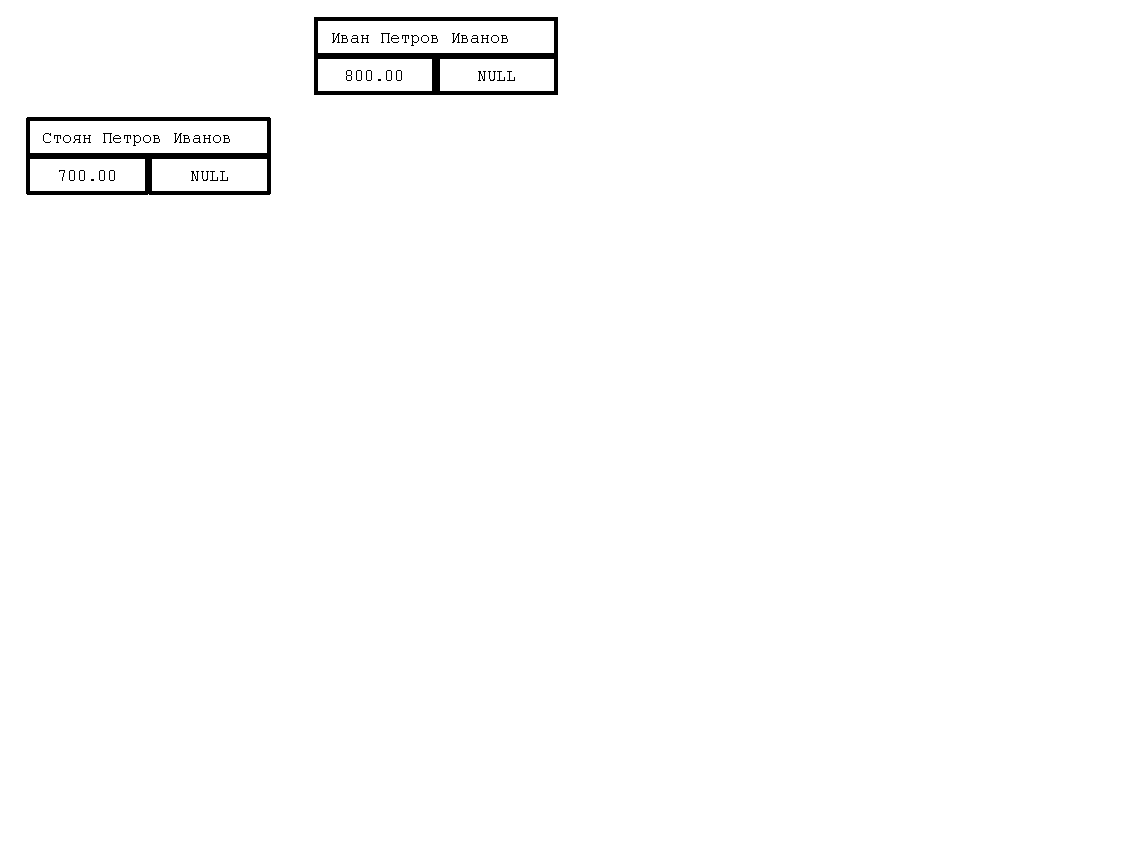
\includegraphics[width=10.5cm]{images/00_rec_obj_two_objects_unlinked}

  \end{column}
\end{columns}
\end{frame}



\begin{frame}[fragile]
\frametitle{Указател към обект от същия тип}

\begin{columns}[c]
  \begin{column}{0.55\textwidth}
\begin{flushleft}
\relscale{0.75}
\begin{lstlisting}

int main ()
{
  Employee 
    stoyan ("Stoyan Petrov Ivanov", 700),
    ivan ("Ivan Petrov Ivanov", 800);

  stoyan.boss = &ivan;

  return 0;
}

\end{lstlisting}  
\end{flushleft}

  \end{column}
  \begin{column}{0.45\textwidth}
\hspace{-100px}
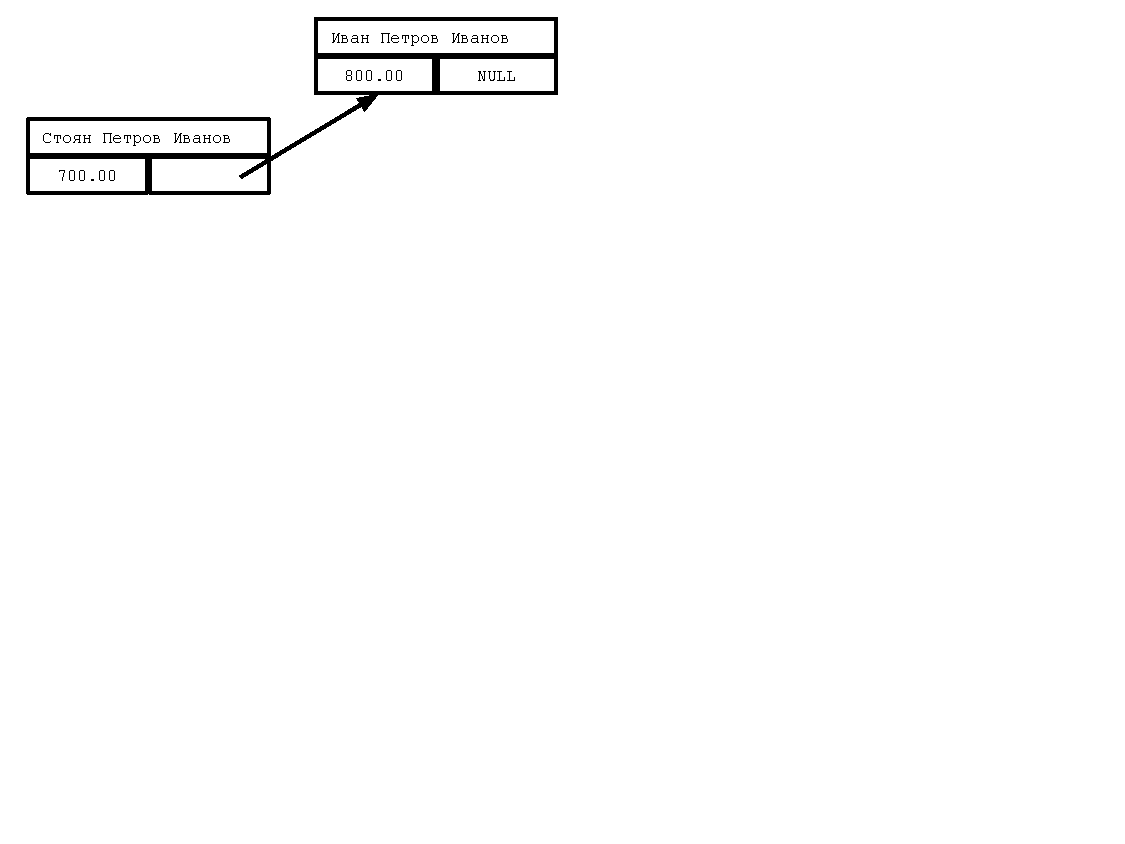
\includegraphics[width=10.5cm]{images/00_rec_obj_two_objects_linked}

  \end{column}
\end{columns}
\end{frame}




\begin{frame}[fragile]
\frametitle{Указател към обект от същия тип}

\begin{columns}[c]
  \begin{column}{0.55\textwidth}
\begin{flushleft}
\relscale{0.75}
\begin{lstlisting}

int main ()
{
  Employee 
    stoyan ("Stoyan Petrov Ivanov", 700),
    ivan ("Ivan Petrov Ivanov", 800),
    bigboss ("Big Boss", 900);

  stoyan.boss = &ivan;
  ivan.boss = &bigboss;
  //stoyan.boss->boss = &bigboss;
  
  cout << stoyan.boss->name;
  cout << stoyan.boss->boss->name;

  return 0;
}

\end{lstlisting}  
\end{flushleft}

  \end{column}
  \begin{column}{0.45\textwidth}
\hspace{-150px}
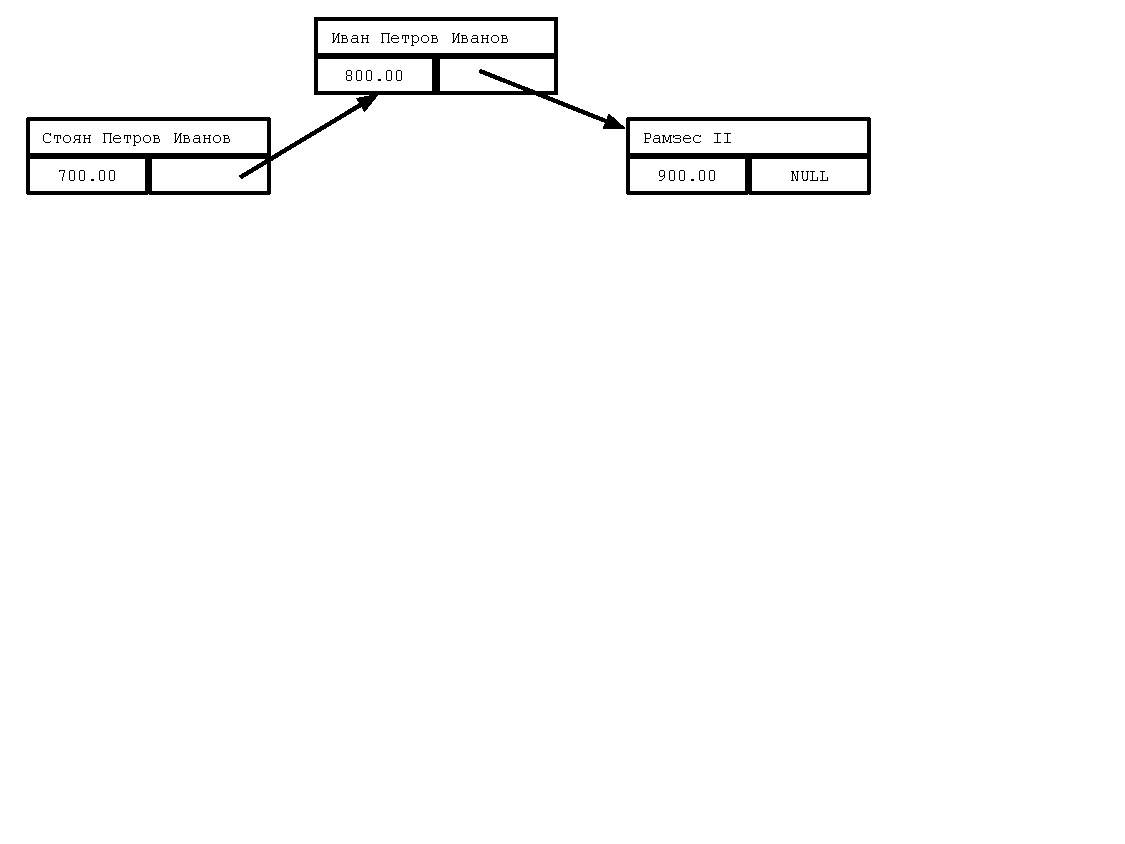
\includegraphics[width=10.5cm]{images/00_rec_obj_three_objects_linked.pdf}

  \end{column}
\end{columns}
\end{frame}



\begin{frame}[fragile]
\frametitle{``Обхождане''}

\begin{columns}[c]
  \begin{column}{0.55\textwidth}
\begin{flushleft}
\relscale{0.75}
\begin{lstlisting}

Employee *findSuperBoss (Employee *e)
{
  while (e->boss != nullptr)
    e = e->boss;
  return e;
}
Employee *findSuperBossRec (Employee *e)
{
  if (e->boss == nullptr)
    return e;
  return findSuperBossRec (e->boss);
}
 //...
 cout << findSuperBoss (&stoyan)->name;
 //...

\end{lstlisting}  
\end{flushleft}

  \end{column}
  \begin{column}{0.45\textwidth}
\hspace{-150px}
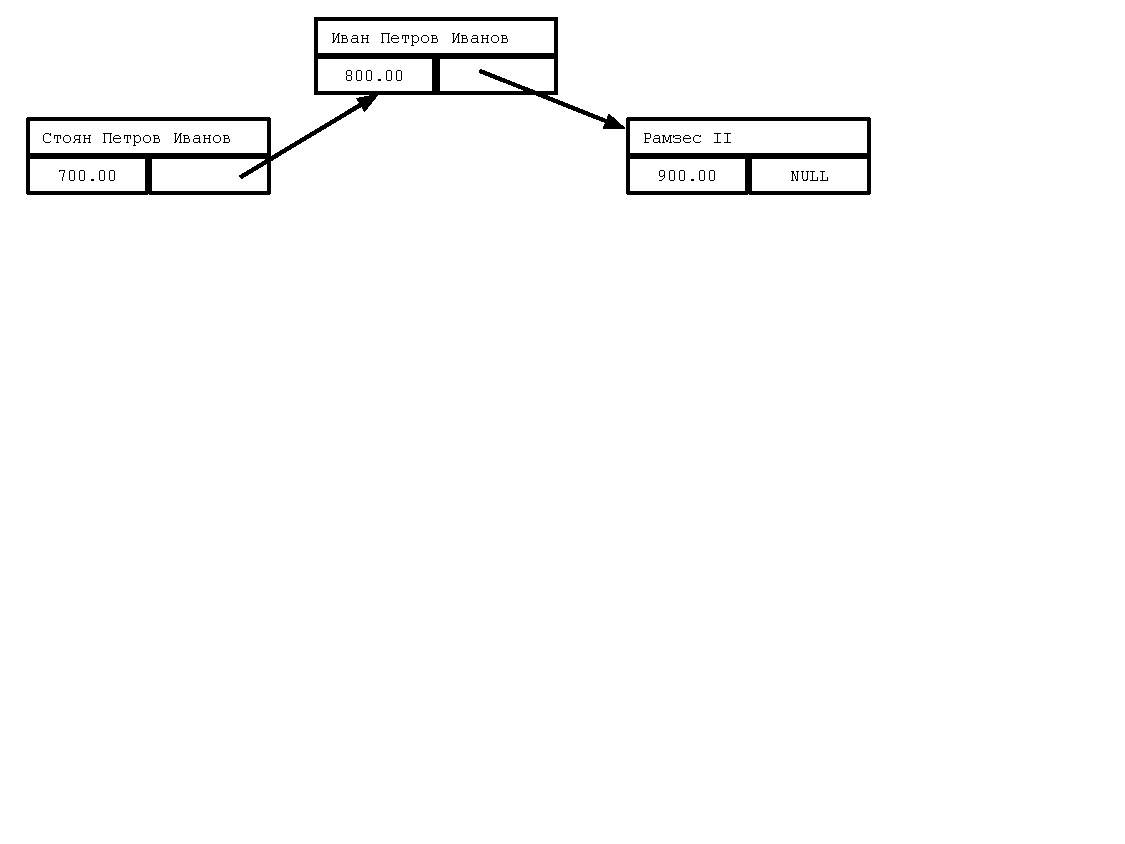
\includegraphics[width=10.5cm]{images/00_rec_obj_three_objects_linked.pdf}

  \end{column}
\end{columns}
\end{frame}



\begin{frame}
\centerline{Линейни едносвързани списъци}
\end{frame}




\begin{frame}[fragile]
\frametitle{Т. нар. ``двойна кутия''}

\begin{flushleft}
\relscale{0.75}
\begin{lstlisting}
struct box
{
  int data;
  box *next;
  box (int d, box *n):
        data(d), next (n) {}
};
\end{lstlisting}  
\end{flushleft}

\begin{itemize}
  \item  Един елемент
\end{itemize}

\begin{flushleft}
\relscale{0.75}
\begin{lstlisting}
box *first = new box (1,nullptr);
\end{lstlisting}  
\end{flushleft}

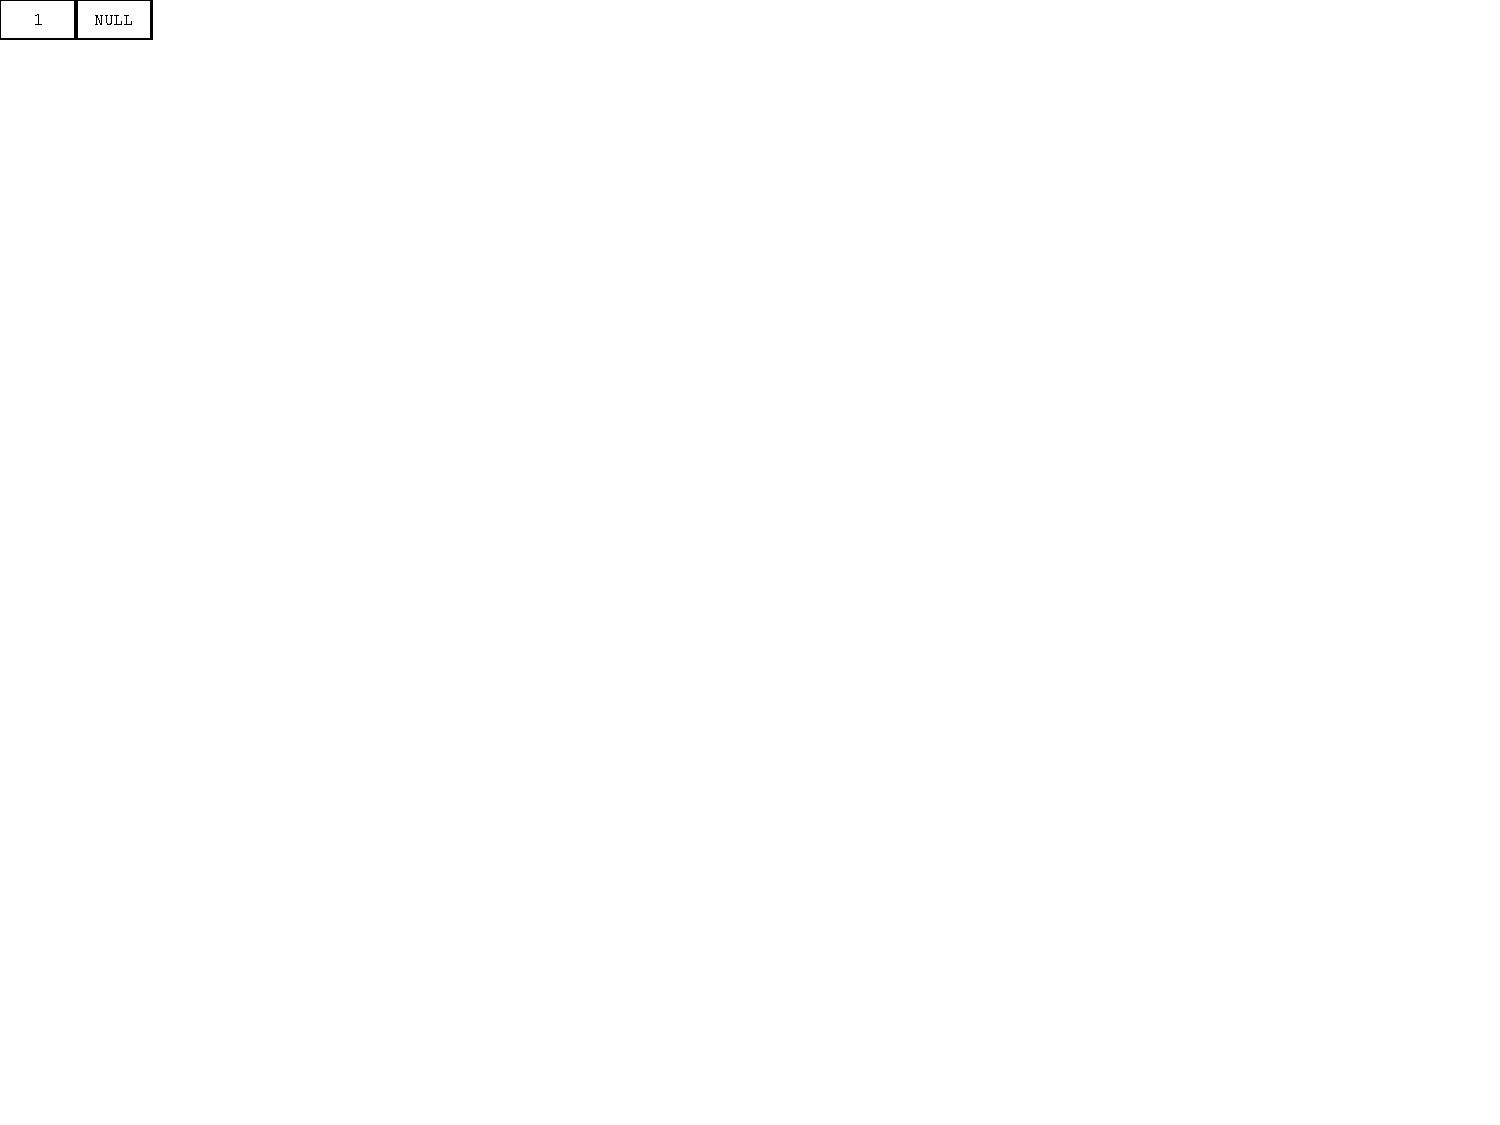
\includegraphics[width=10.5cm]{images/01_llbox_onebox.pdf}

\vspace{-210px}

\begin{itemize}
  \item  Два свързани елемента
\end{itemize}

\begin{flushleft}
\relscale{0.75}
\begin{lstlisting}
box *first = new box (1,new box (2, nullptr));
\end{lstlisting}  
\end{flushleft}

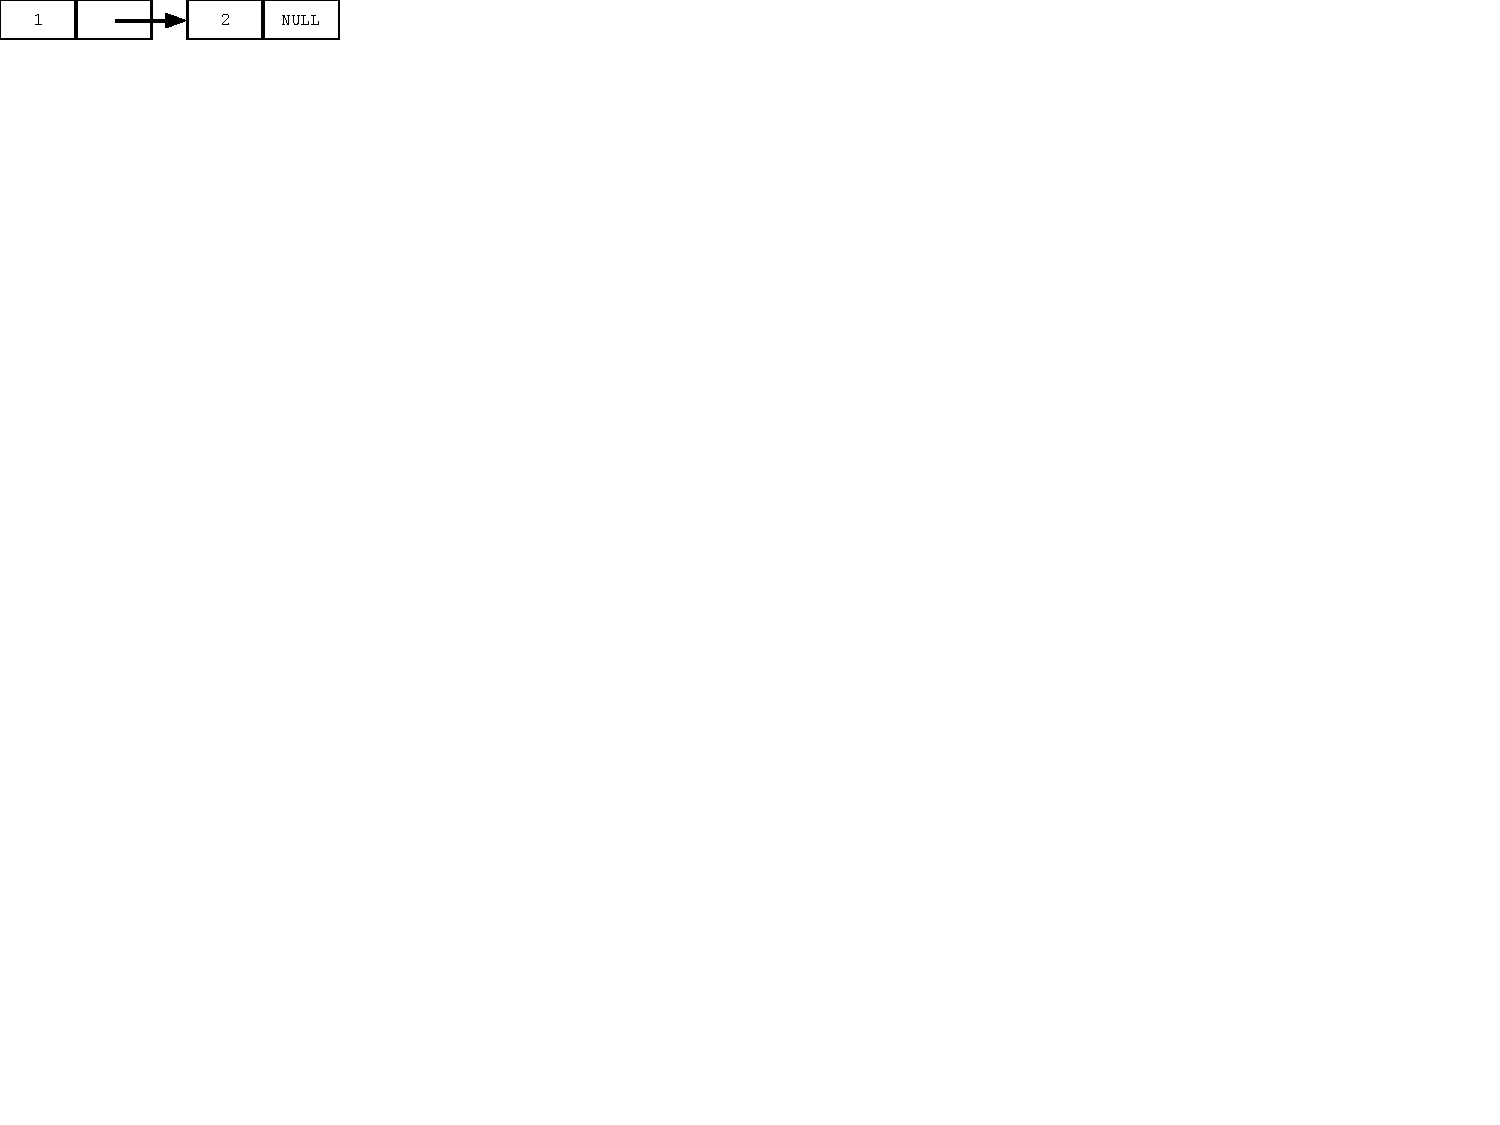
\includegraphics[width=10.5cm]{images/01_llbox_twoboxes.pdf}


\end{frame}


\begin{frame}[fragile]
\frametitle{``Плосък'' изглед}

\begin{flushleft}
\relscale{0.75}
\begin{lstlisting}
box *first = new box (1,
               new box (2, 
                new box (3, 
                  new box (4, 
                    new box (5,nullptr)))));
\end{lstlisting}  
\end{flushleft}


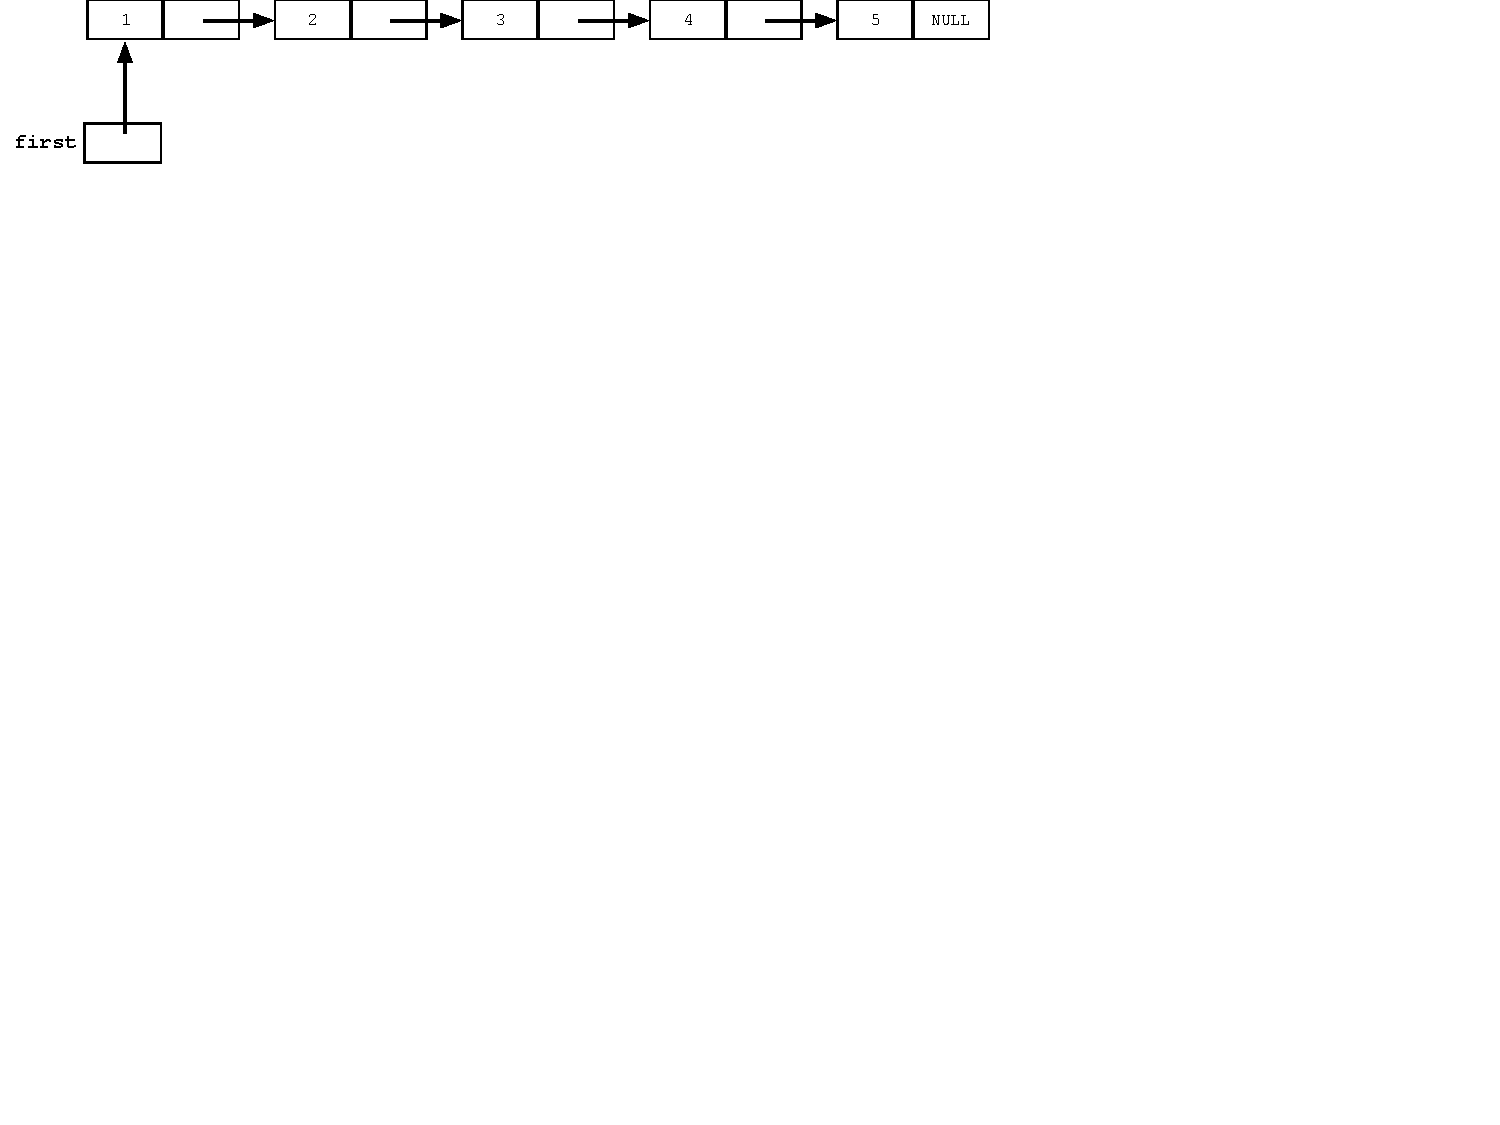
\includegraphics[width=14.0cm]{images/02_ll_flatchain}

\end{frame}



\begin{frame}[fragile]
\frametitle{``Реален'' изглед}

\begin{flushleft}
\relscale{0.75}
\begin{lstlisting}
box *first = new box (1,
               new box (2, 
                new box (3, 
                  new box (4, 
                    new box (5,nullptr)))));
\end{lstlisting}  
\end{flushleft}


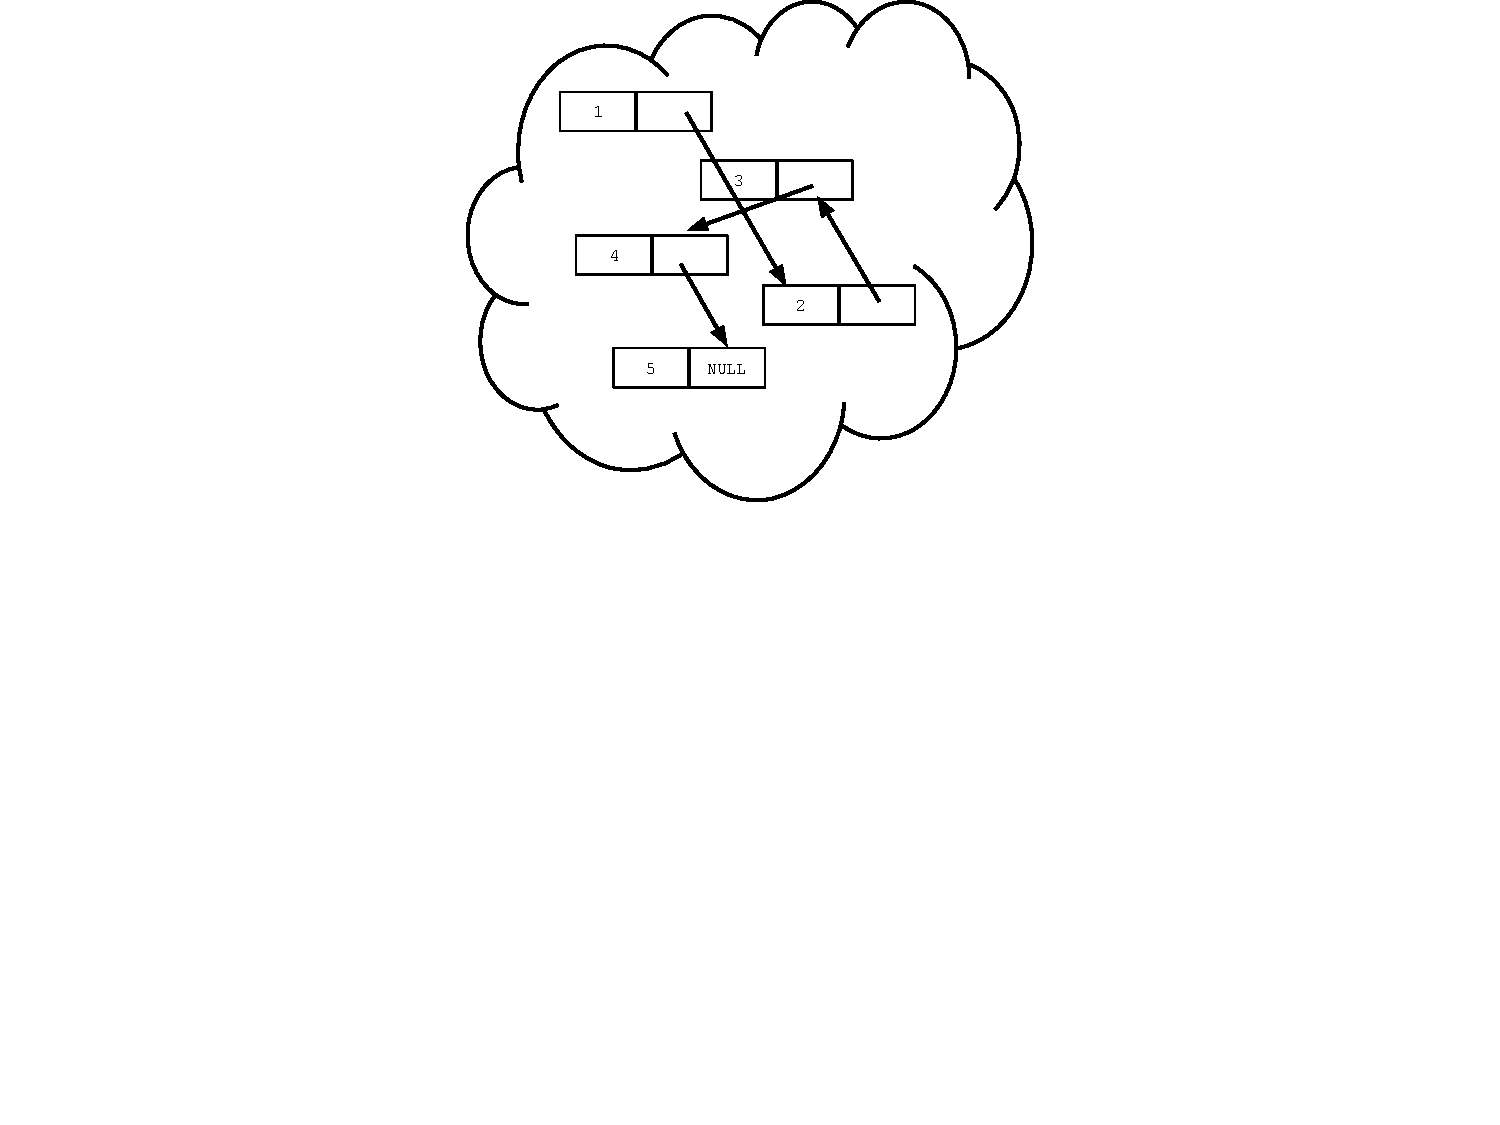
\includegraphics[width=14.0cm]{images/02_ll_boxcloud}

\end{frame}



\begin{frame}
\centerline{``Вмъкване'' на елемент в началото (push)}
\end{frame}



\begin{frame}[fragile]
\frametitle{``Вмъкване'' на елемент в началото}

\begin{flushleft}
\relscale{0.75}
\begin{lstlisting}
first = ...
\end{lstlisting}  
\end{flushleft}


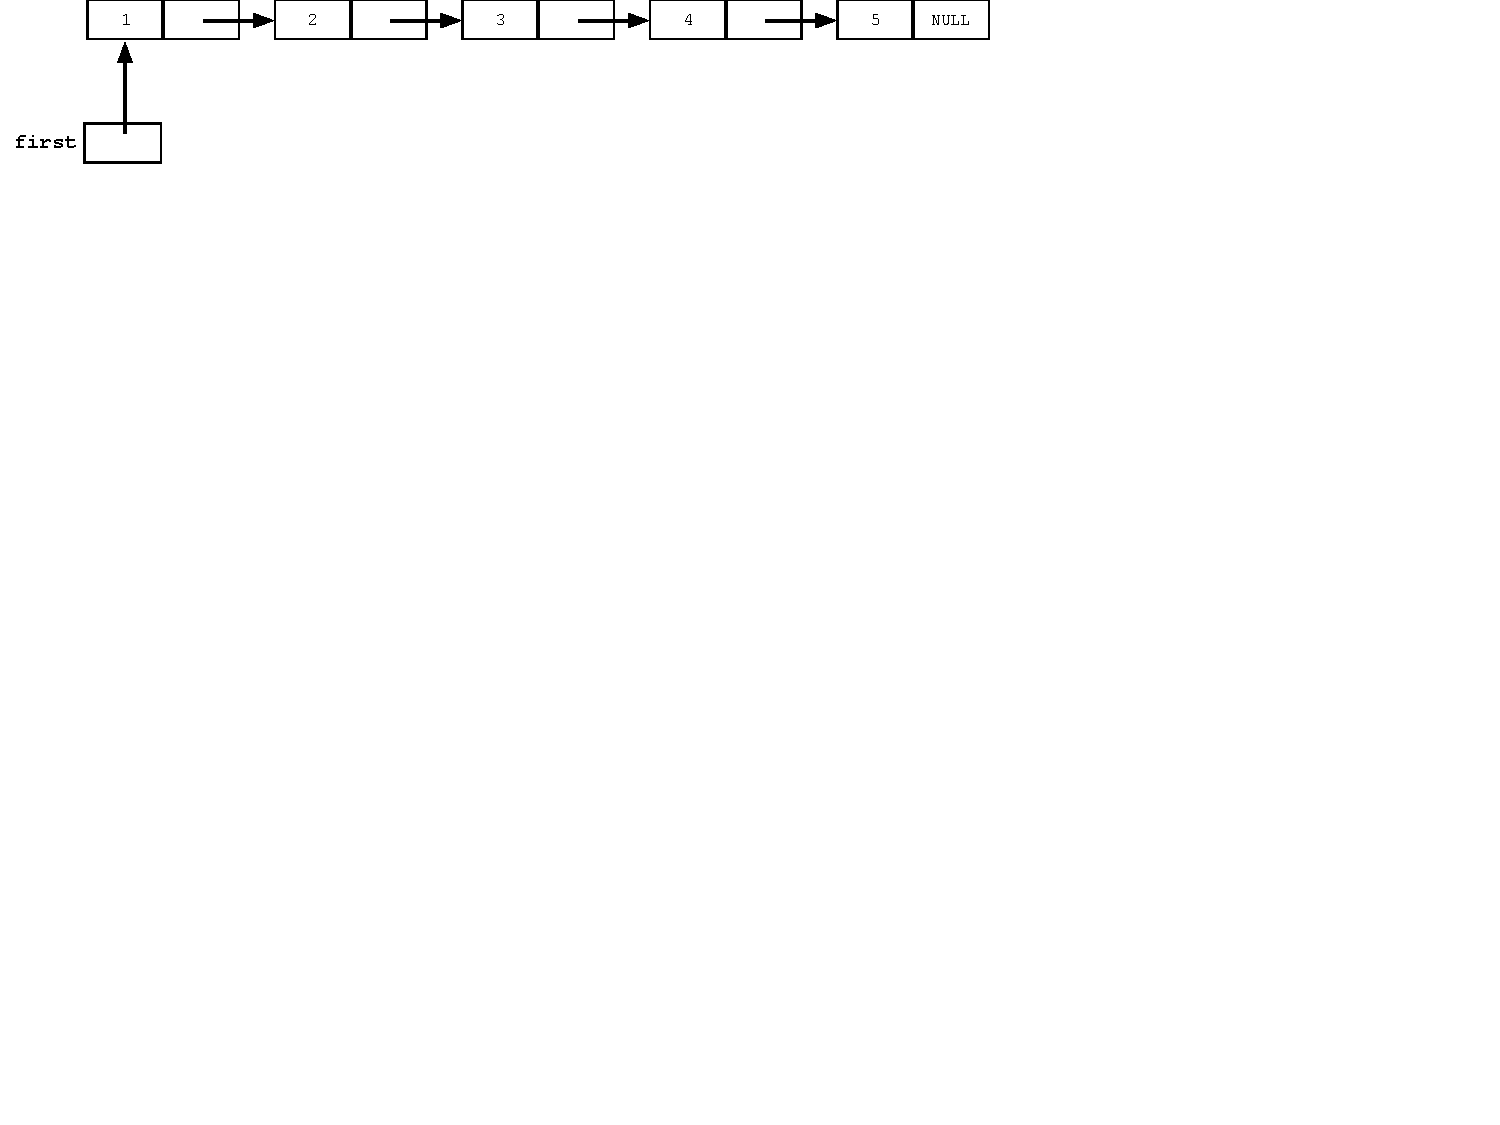
\includegraphics[width=14.0cm]{images/02_ll_flatchain}

\end{frame}


\begin{frame}[fragile]
\frametitle{``Вмъкване'' на елемент в началото}

\begin{flushleft}
\relscale{0.75}
\begin{lstlisting}
box *newbox = new box (7,nullptr);
\end{lstlisting}  
\end{flushleft}


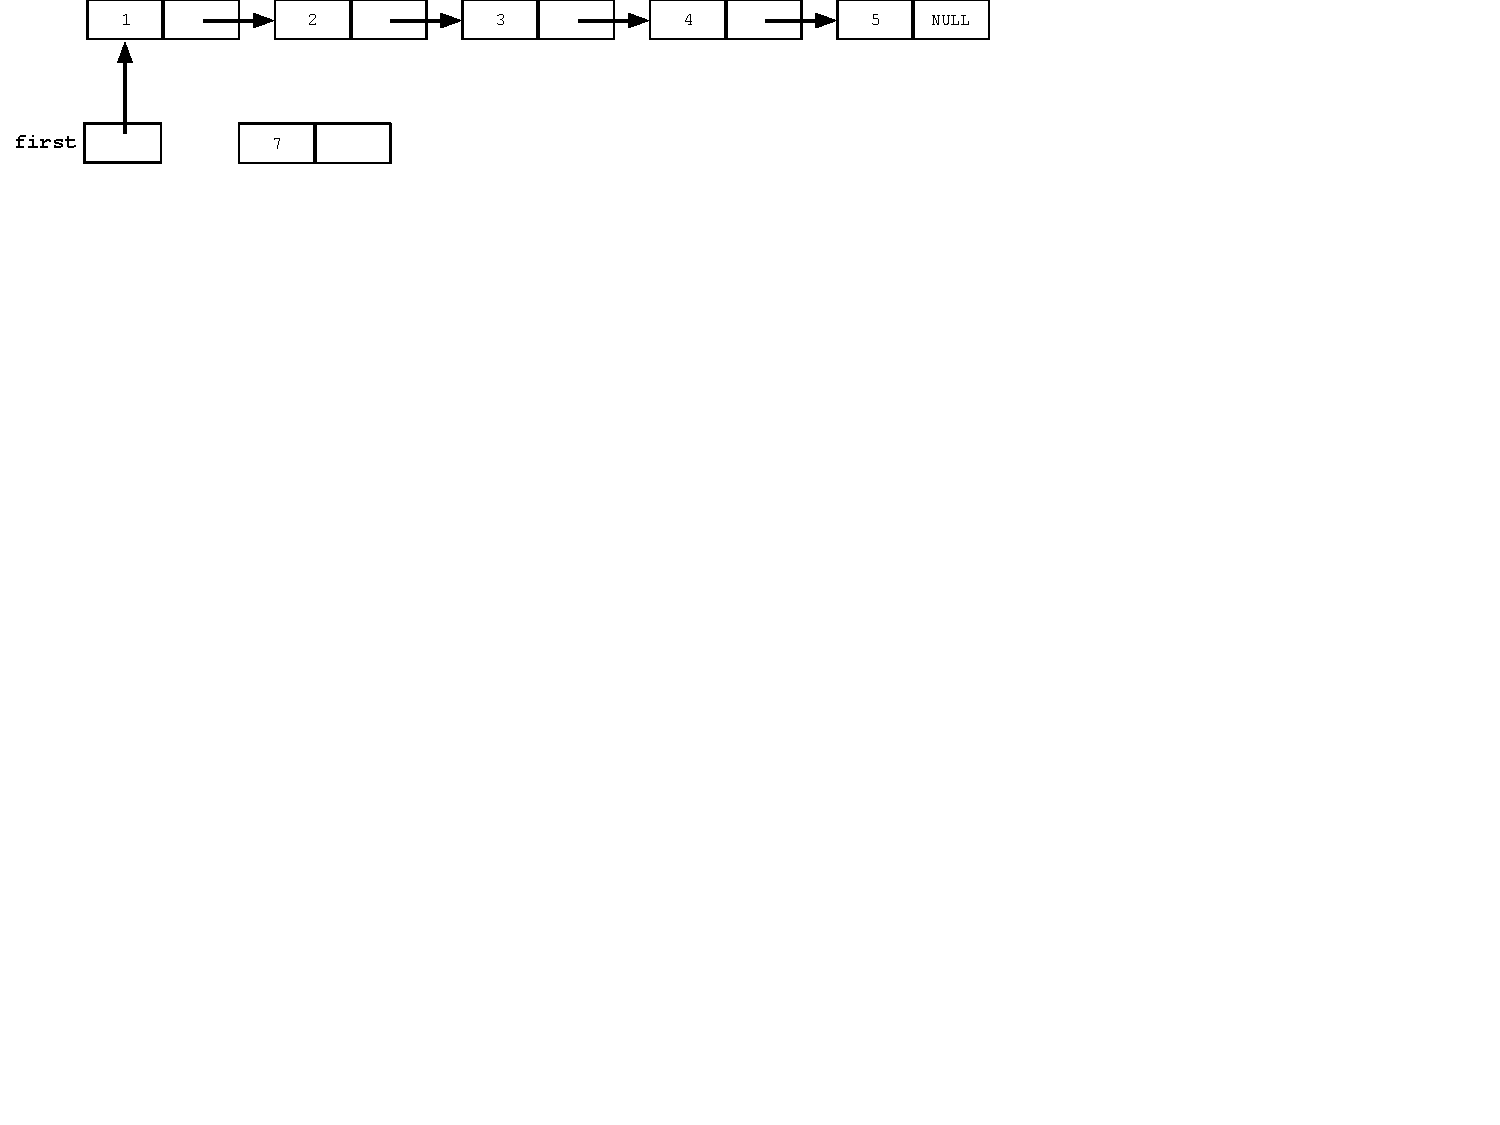
\includegraphics[width=14.0cm]{images/03_ll_push_initial}

\end{frame}

\begin{frame}[fragile]
\frametitle{``Вмъкване'' на елемент в началото}

\begin{flushleft}
\relscale{0.75}
\begin{lstlisting}
box *newbox = new box (7,nullptr);
newbox->next = first;
\end{lstlisting}  
\end{flushleft}


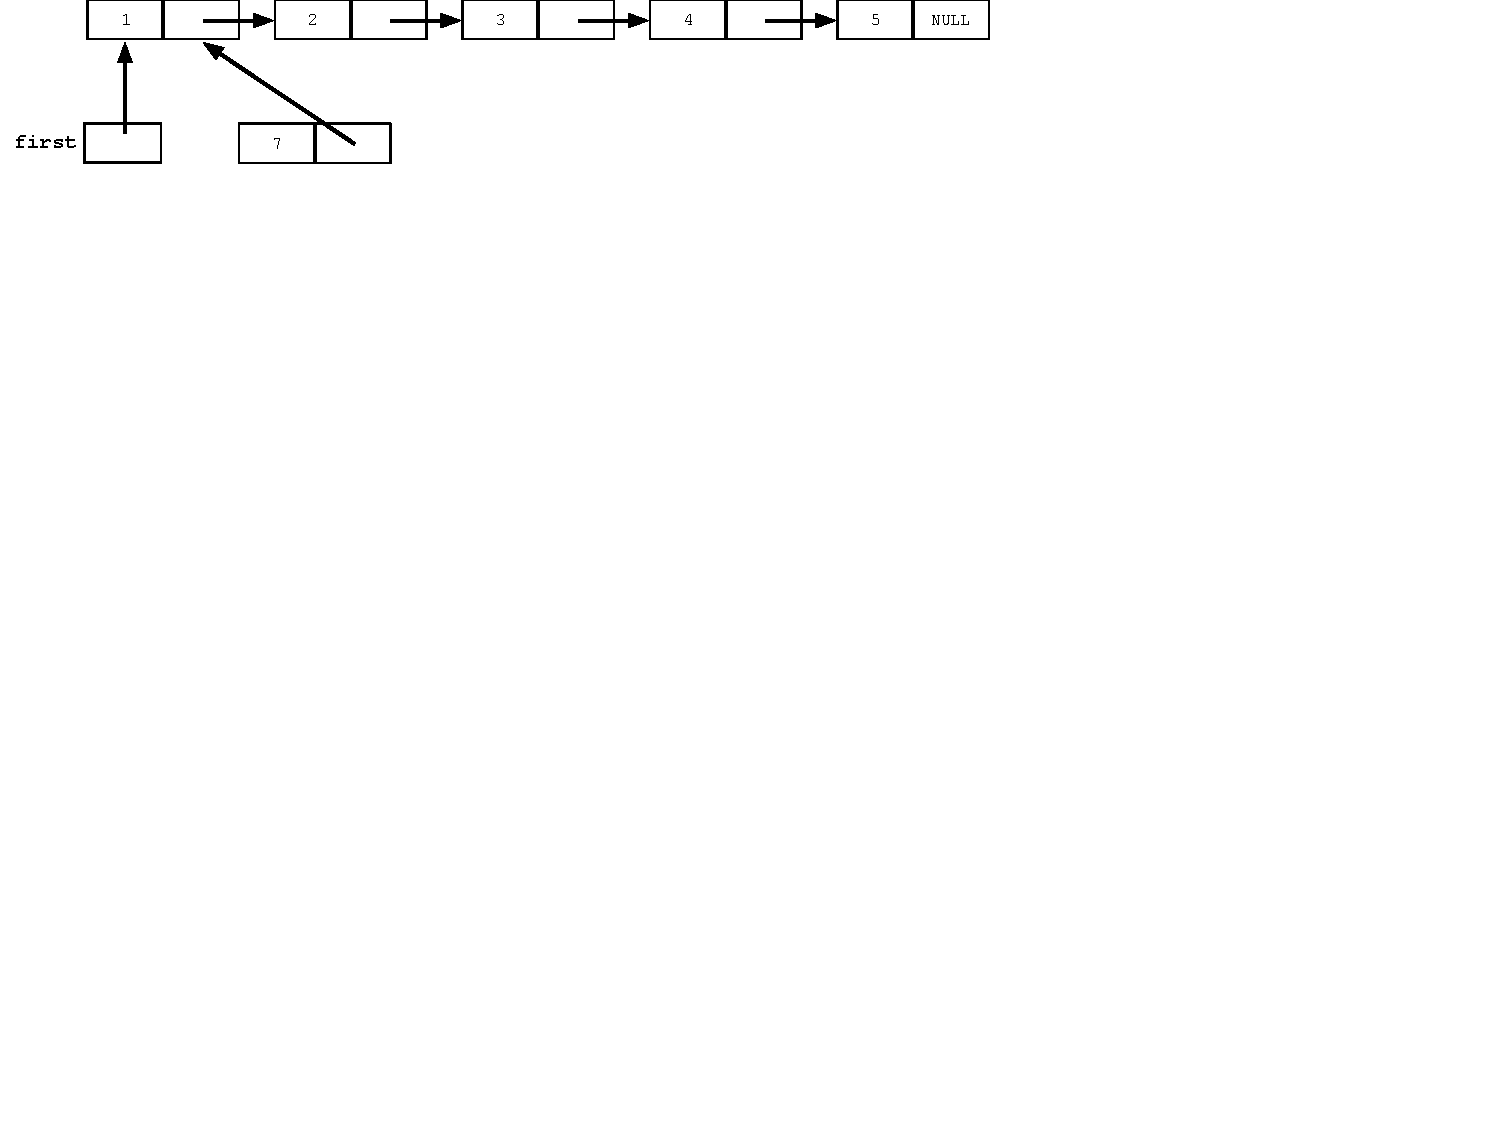
\includegraphics[width=14.0cm]{images/03_ll_push_firstlink.pdf}

\end{frame}



\begin{frame}[fragile]
\frametitle{``Вмъкване'' на елемент в началото}

\begin{flushleft}
\relscale{0.75}
\begin{lstlisting}
box *newbox = new box (7,nullptr);
newbox->next = first;
first = newbox;
\end{lstlisting}  
\end{flushleft}


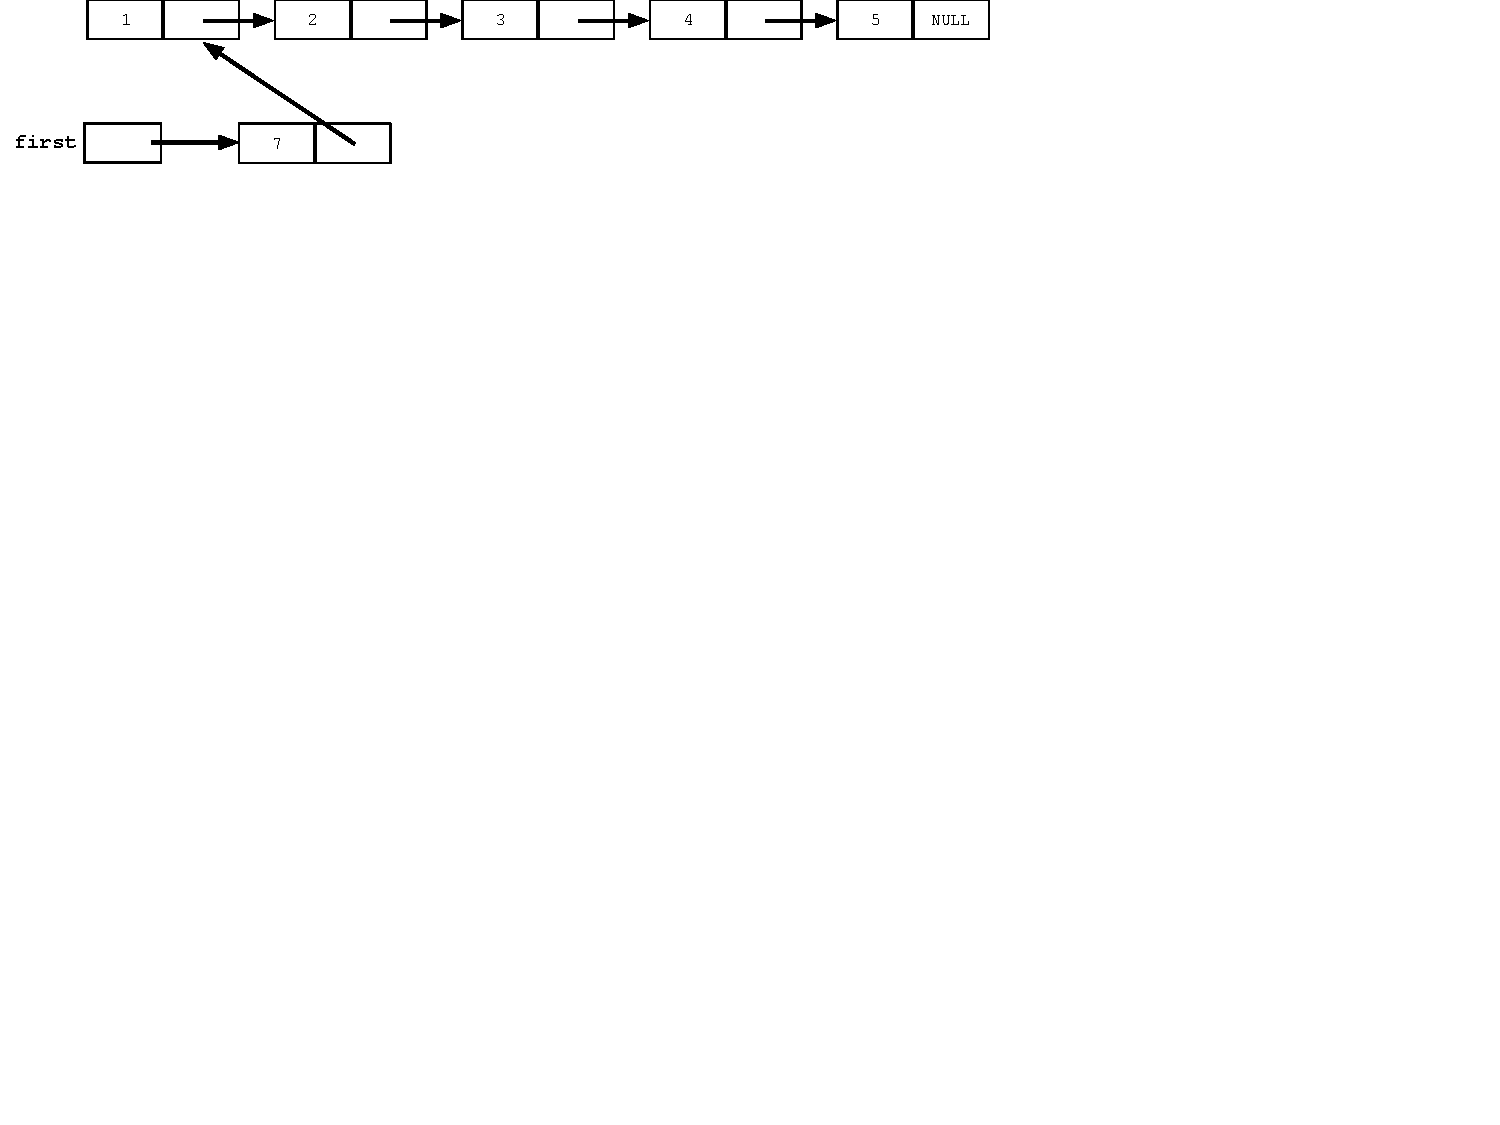
\includegraphics[width=14.0cm]{images/03_ll_push_secondtlink.pdf}

\end{frame}



\begin{frame}
\centerline{Обхождане}
\end{frame}



\begin{frame}[fragile]
\frametitle{Обхождане на всички елементи}

\begin{flushleft}
\relscale{0.75}
\begin{lstlisting}
cout << first->data;
\end{lstlisting}  
\end{flushleft}


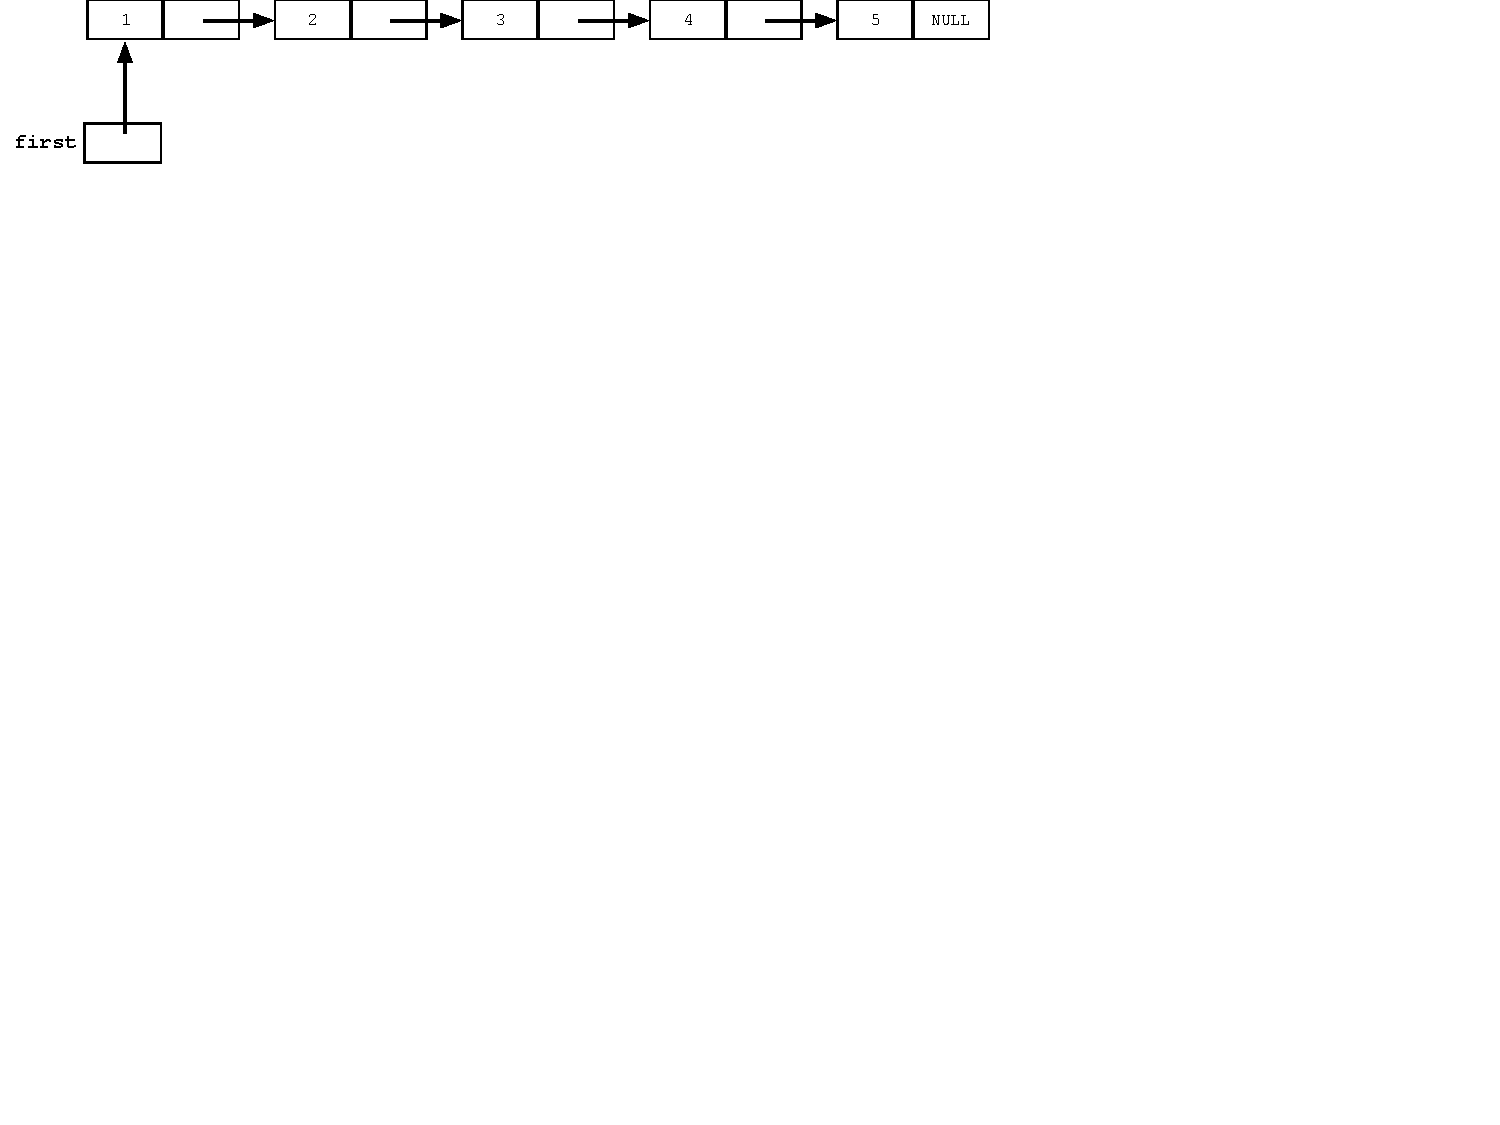
\includegraphics[width=14.0cm]{images/02_ll_flatchain}

\end{frame}

\begin{frame}[fragile]
\frametitle{Обхождане на всички елементи}

\begin{itemize}
  \item Трябва ни помощен указател!  
\end{itemize}

\begin{flushleft}
\relscale{0.75}
\begin{lstlisting}
first = first->next;
cout << first->data;
\end{lstlisting}  
\end{flushleft}


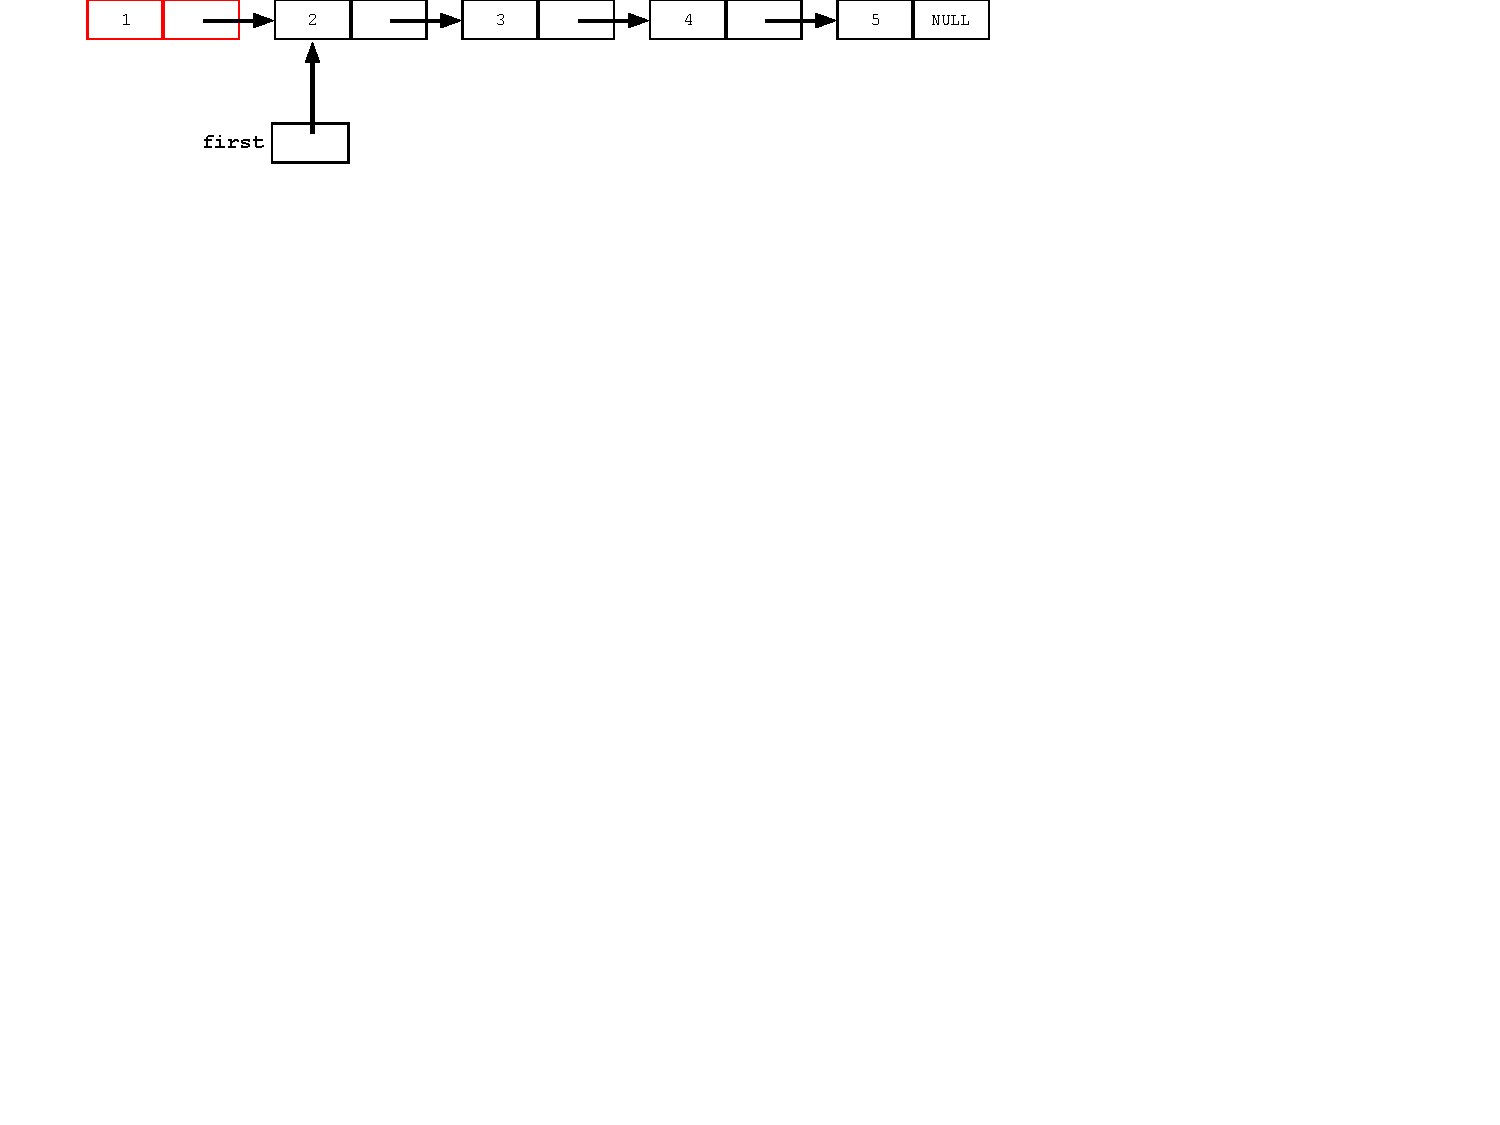
\includegraphics[width=14.0cm]{images/06_ll_pop}

\end{frame}



\begin{frame}[fragile]
\frametitle{Обхождане на всички елементи}

\begin{flushleft}
\relscale{0.75}
\begin{lstlisting}
box *crr = first;
cout << crr->data;
\end{lstlisting}  
\end{flushleft}


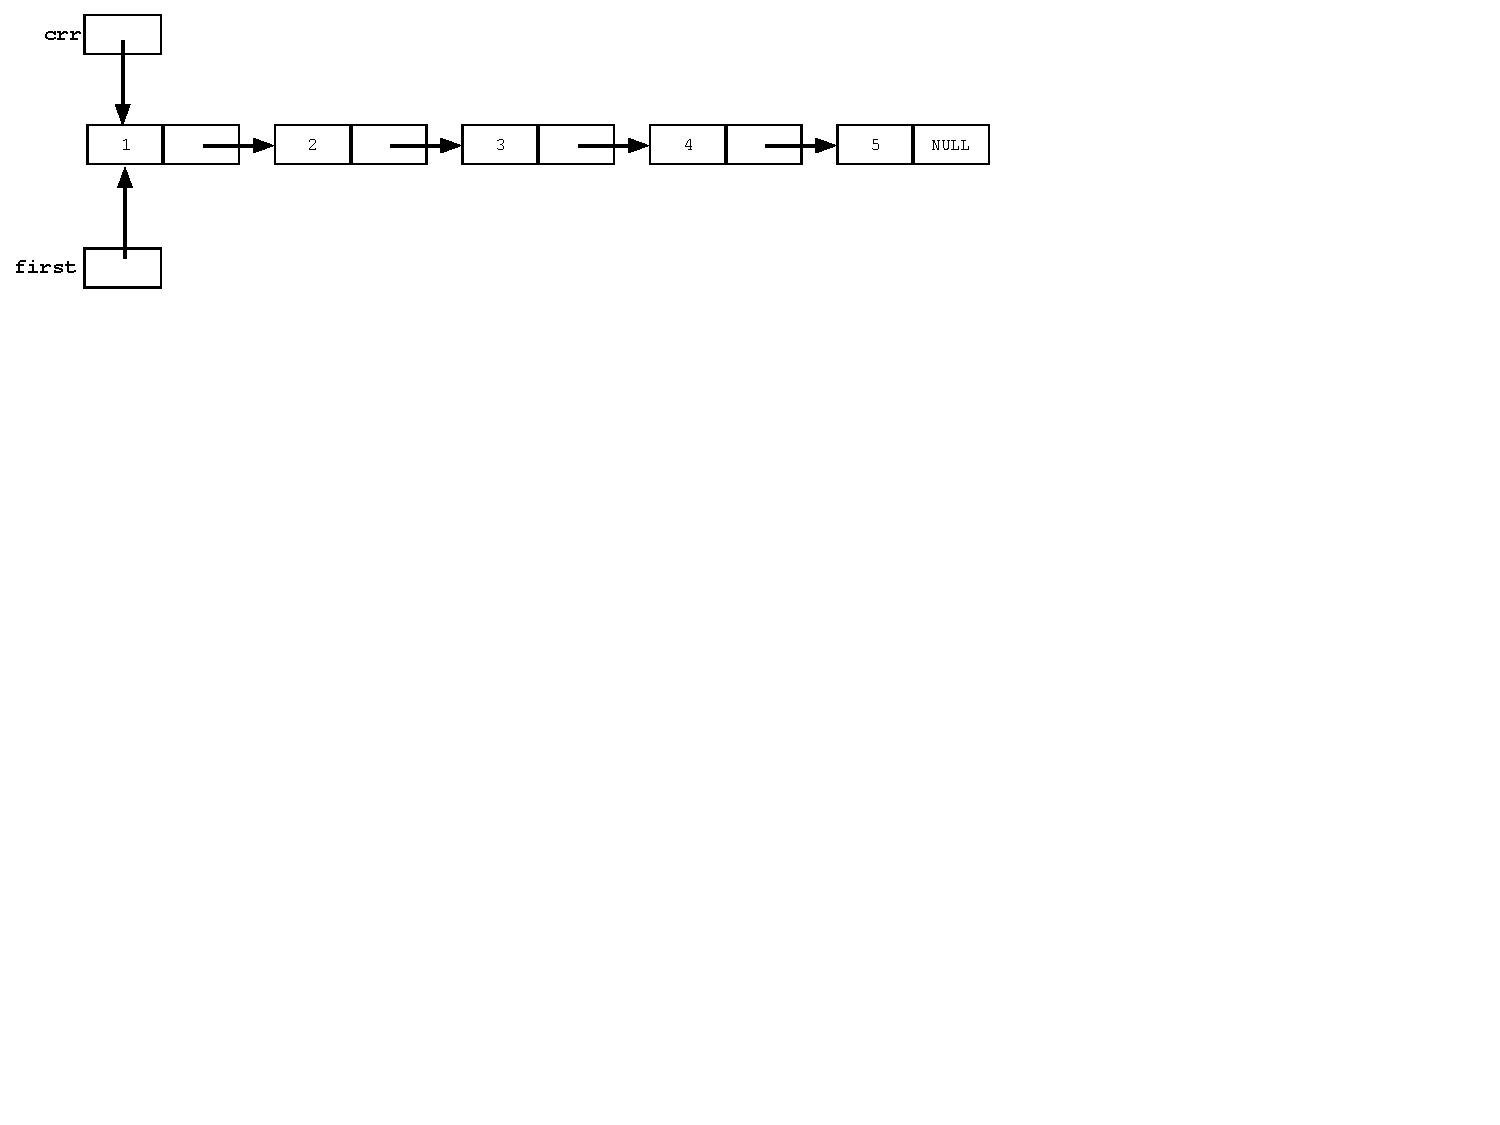
\includegraphics[width=14.0cm]{images/04_ll_trav_start}

\end{frame}


\begin{frame}[fragile]
\frametitle{Обхождане на всички елементи}

\begin{flushleft}
\relscale{0.75}
\begin{lstlisting}
box *crr = first;
crr = crr->next;
cout << crr->data;
\end{lstlisting}  
\end{flushleft}


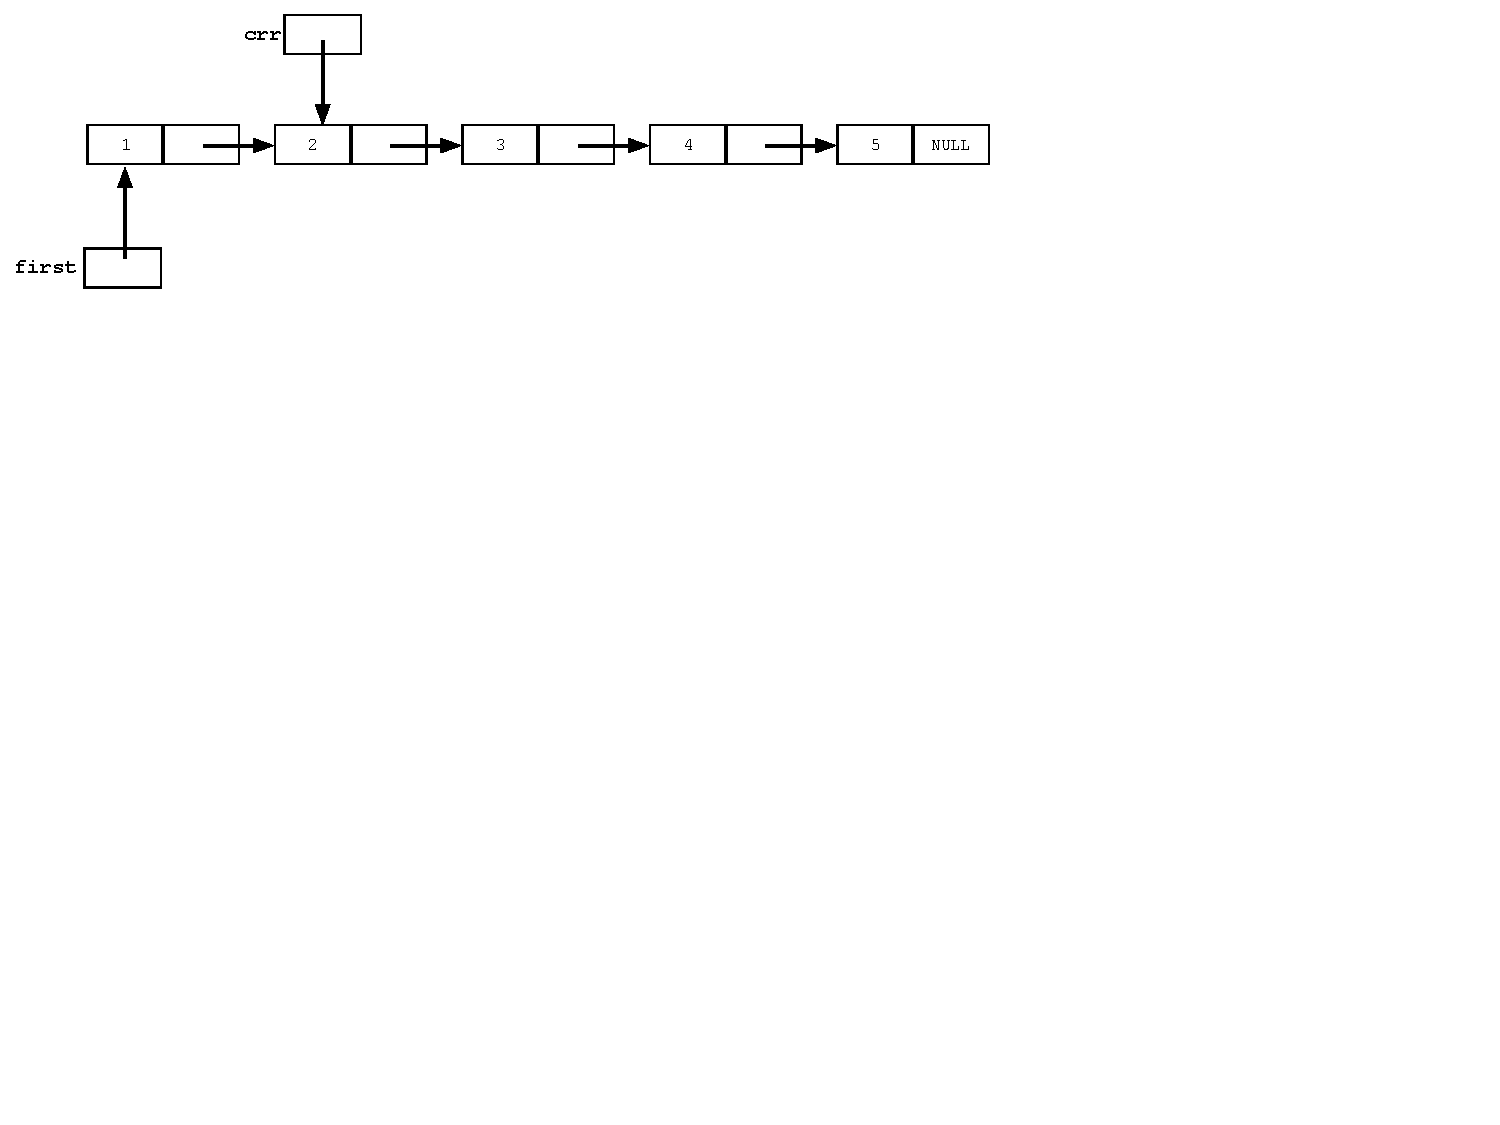
\includegraphics[width=14.0cm]{images/04_ll_trav_stepone}

\end{frame}

\begin{frame}[fragile]
\frametitle{Обхождане на всички елементи}

\begin{flushleft}
\relscale{0.75}
\begin{lstlisting}
box *crr = first;
while (crr != nullptr)
{
  cout << crr->data;
  crr = crr->next;
}
\end{lstlisting}  
\end{flushleft}


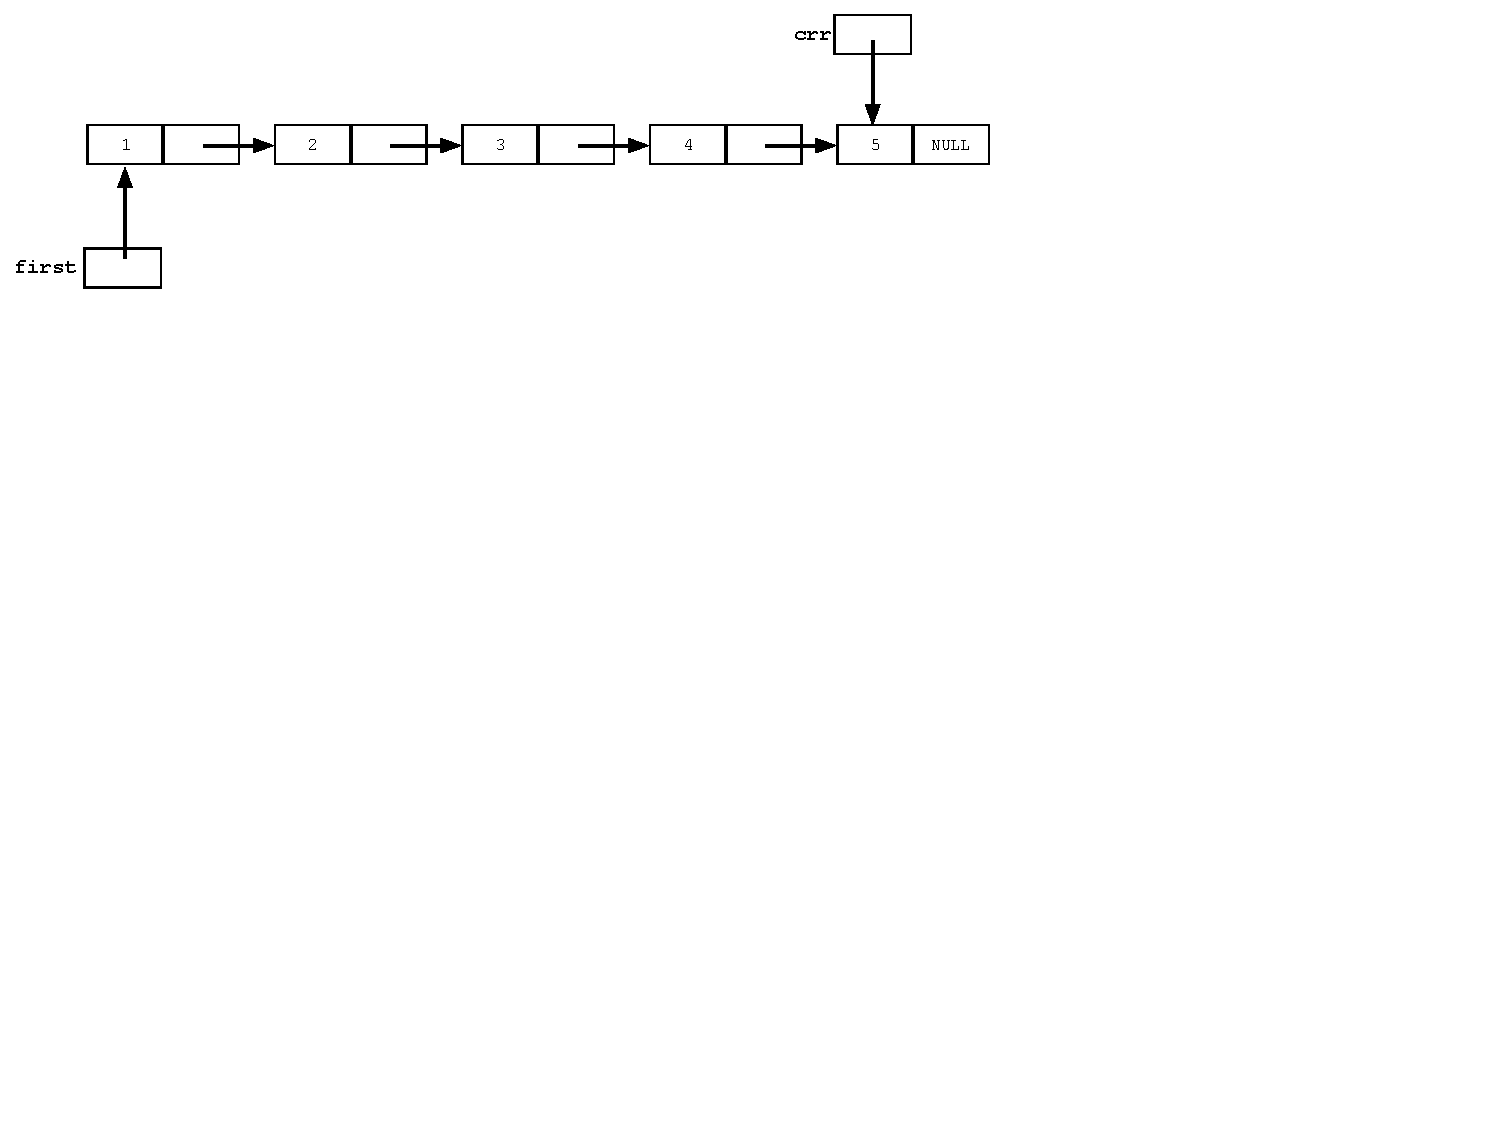
\includegraphics[width=14.0cm]{images/04_ll_trav_eol}

\end{frame}


\begin{frame}
\centerline{Вмъкване във вътрешността}
\end{frame}



\begin{frame}[fragile]
\frametitle{Вмъкване}

\begin{flushleft}
\relscale{0.75}
\begin{lstlisting}
box *newbox = new box (7,nullptr);
\end{lstlisting}  
\end{flushleft}


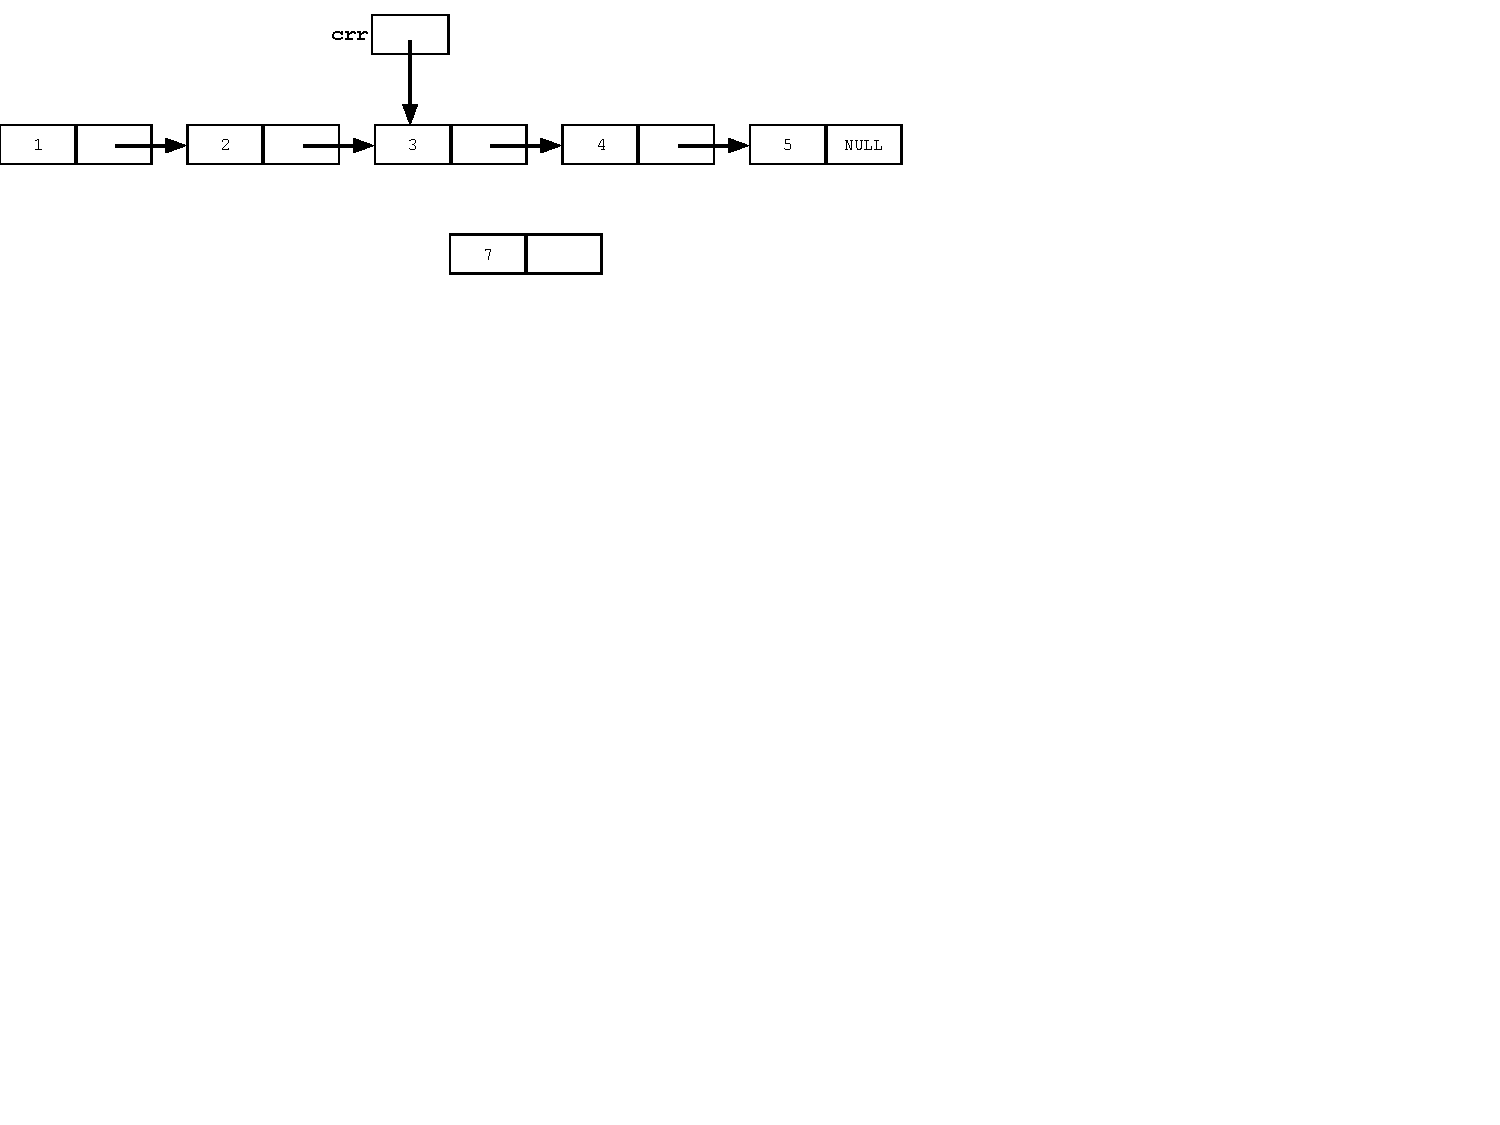
\includegraphics[width=14.0cm]{images/05_ll_insert_start}

\end{frame}

\begin{frame}[fragile]
\frametitle{Вмъкване}

\begin{flushleft}
\relscale{0.75}
\begin{lstlisting}
box *newbox = new box (7,nullptr);
newbox->next = crr->next;
\end{lstlisting}  
\end{flushleft}


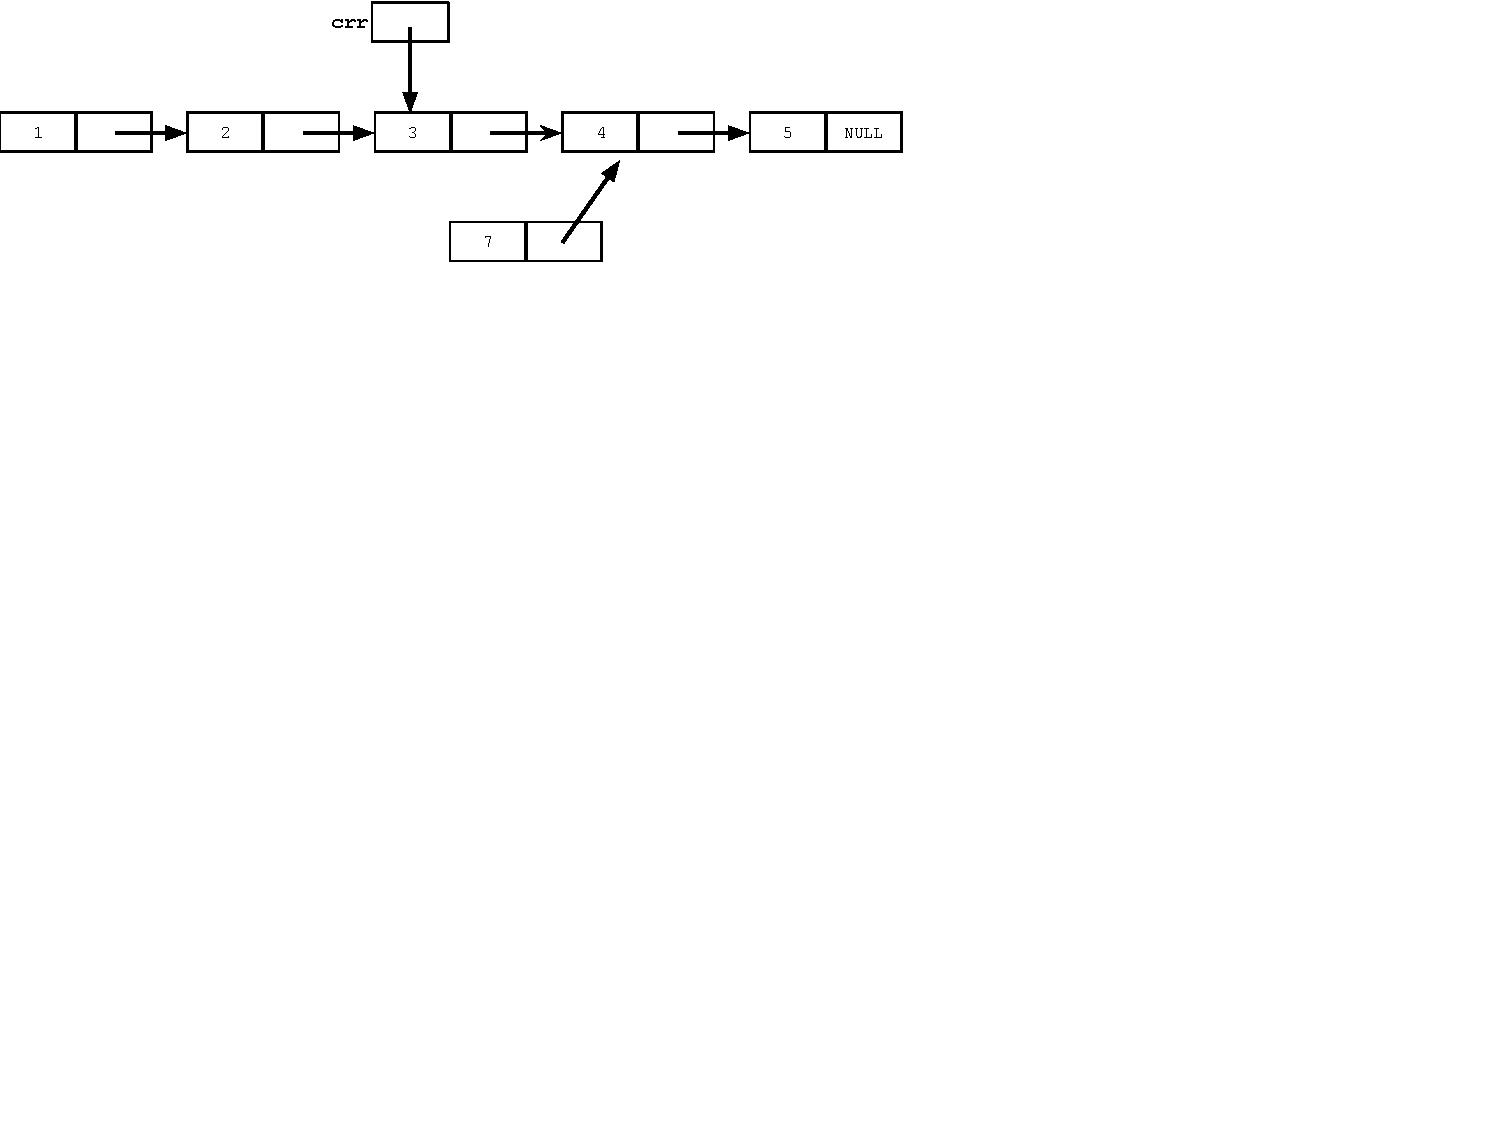
\includegraphics[width=14.0cm]{images/05_ll_insert_firstlink}

\end{frame}


\begin{frame}[fragile]
\frametitle{Вмъкване}

\begin{flushleft}
\relscale{0.75}
\begin{lstlisting}
box *newbox = new box (7,nullptr);
newbox->next = crr->next;
crr->next = newbox;
\end{lstlisting}  
\end{flushleft}


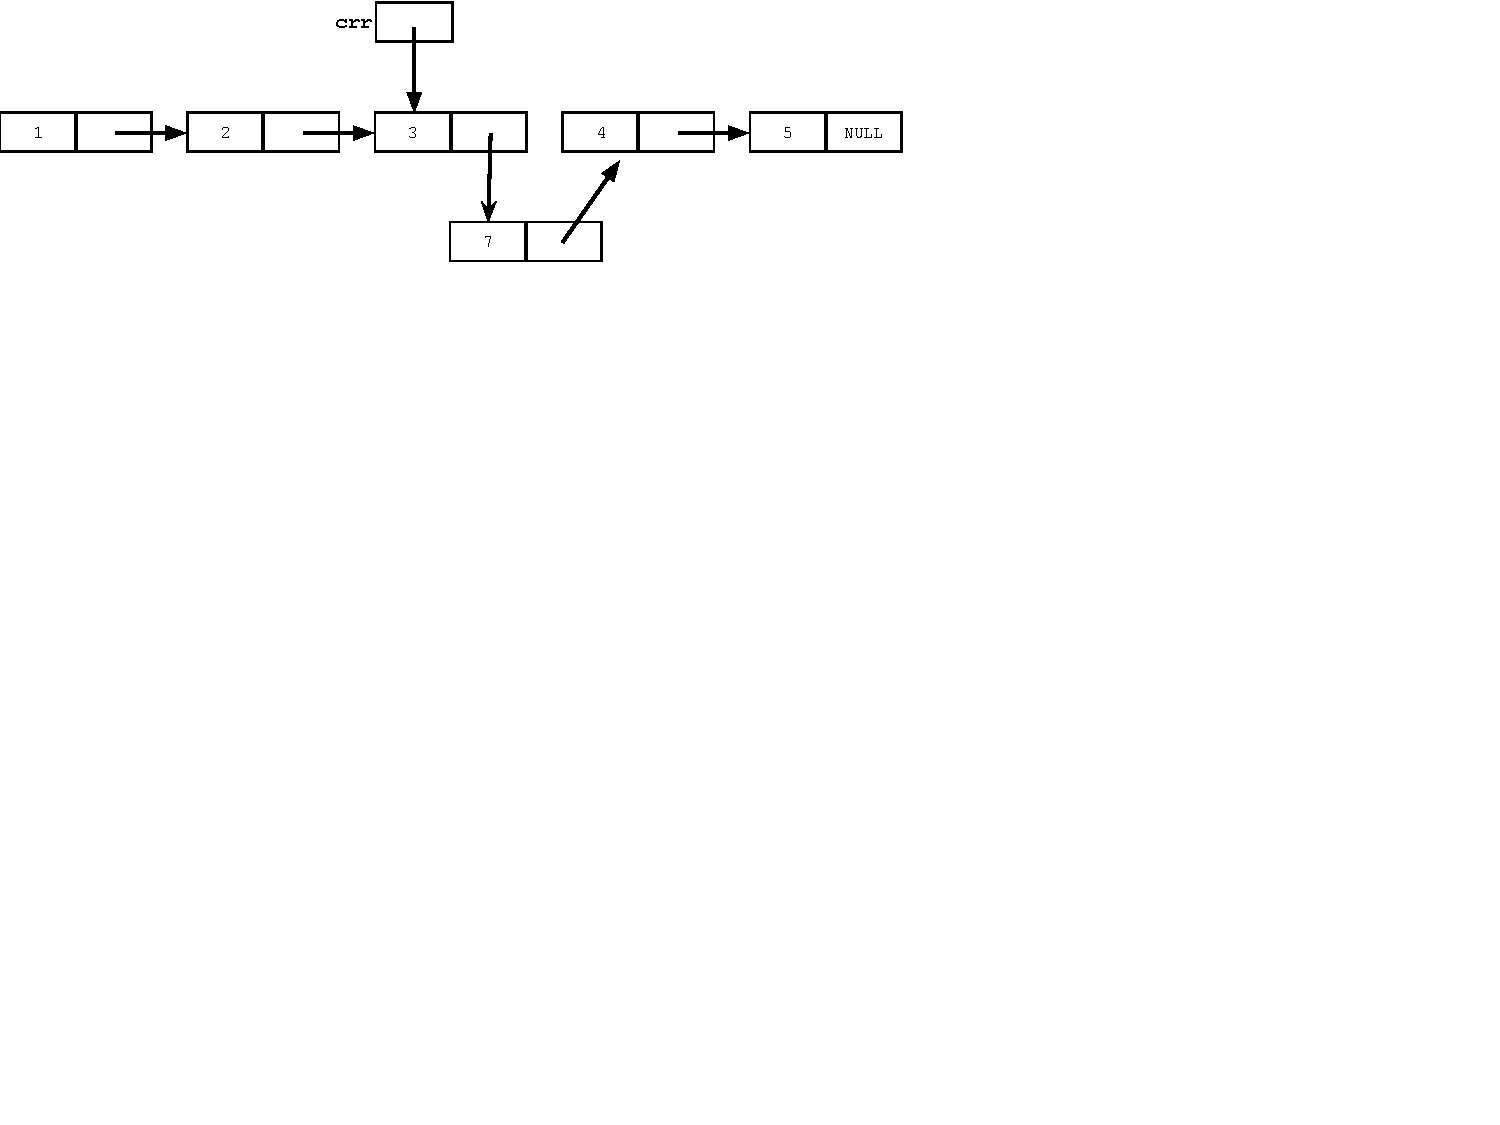
\includegraphics[width=14.0cm]{images/05_ll_insert_secondlink}

\end{frame}



\begin{frame}[fragile]
\frametitle{Вмъкване}

\begin{flushleft}
\relscale{0.75}
\begin{lstlisting}
box *crr = first;
while (3 != crr->data)
  crr = crr->next;

box *newbox = new box (7,nullptr);
newbox->next = crr->next;
crr->next = newbox;
\end{lstlisting}  
\end{flushleft}


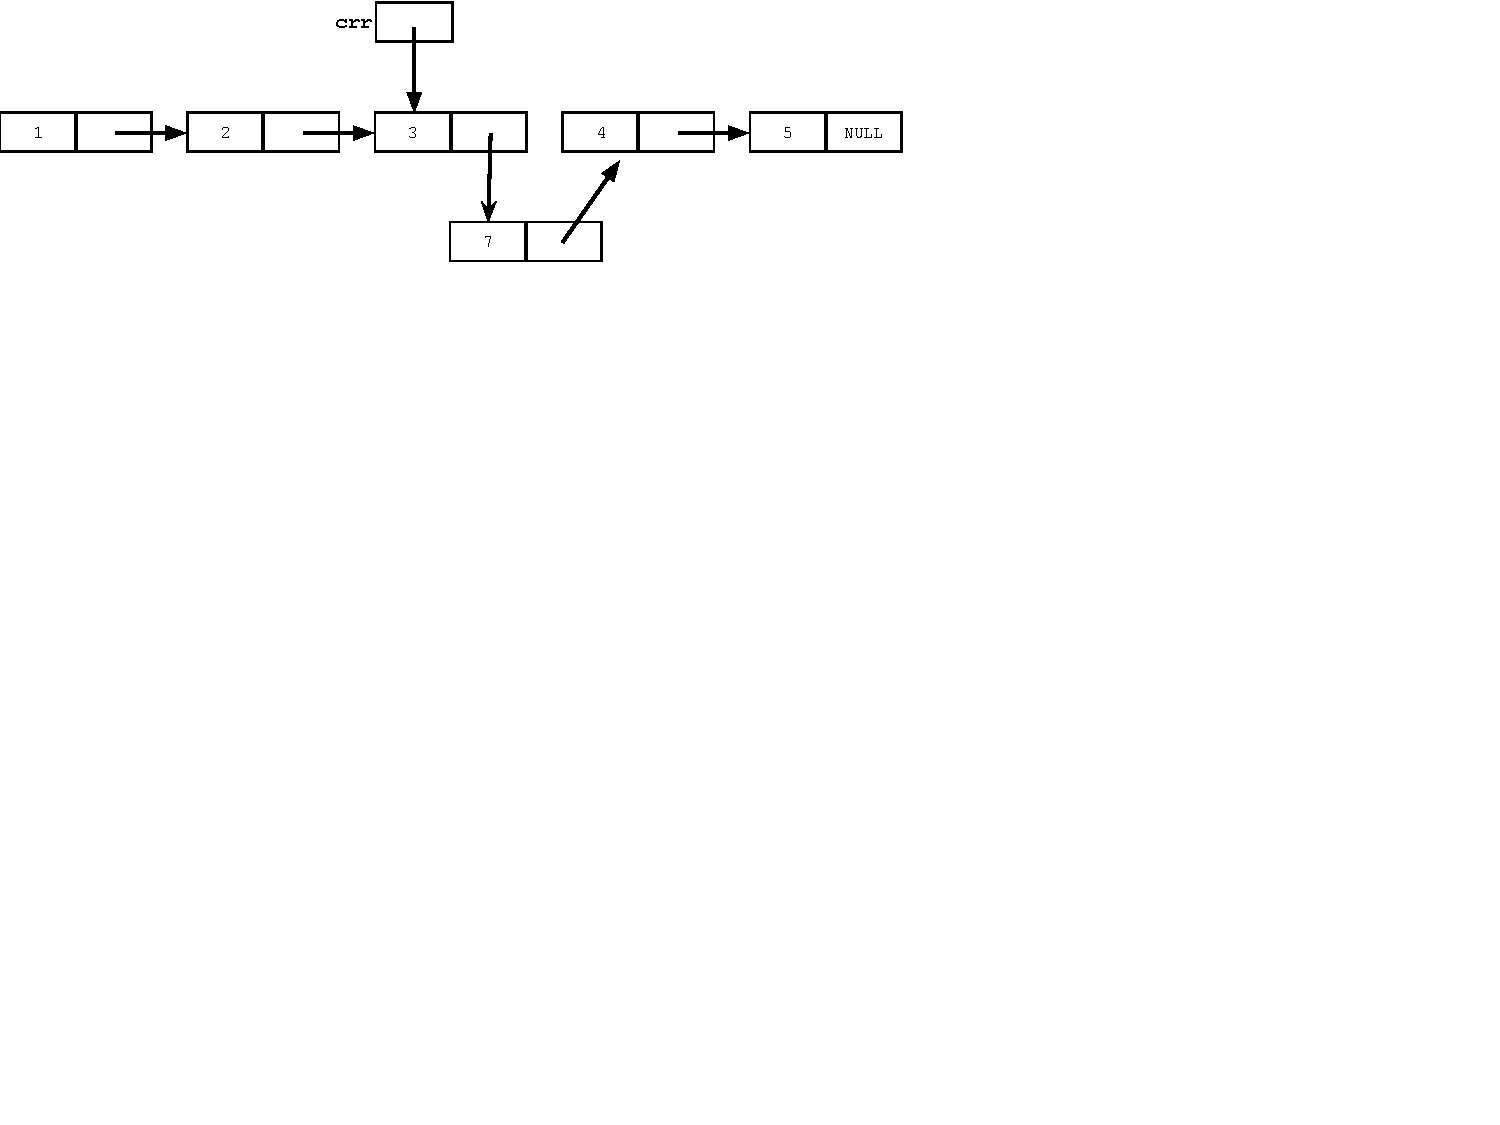
\includegraphics[width=14.0cm]{images/05_ll_insert_secondlink}

\end{frame}



\begin{frame}
\centerline{Изтриване на елемент от началото (pop)}
\end{frame}



\begin{frame}[fragile]
\frametitle{Pop}

\begin{flushleft}
\relscale{0.75}
\begin{lstlisting}
first=first->next;
\end{lstlisting}  
\end{flushleft}


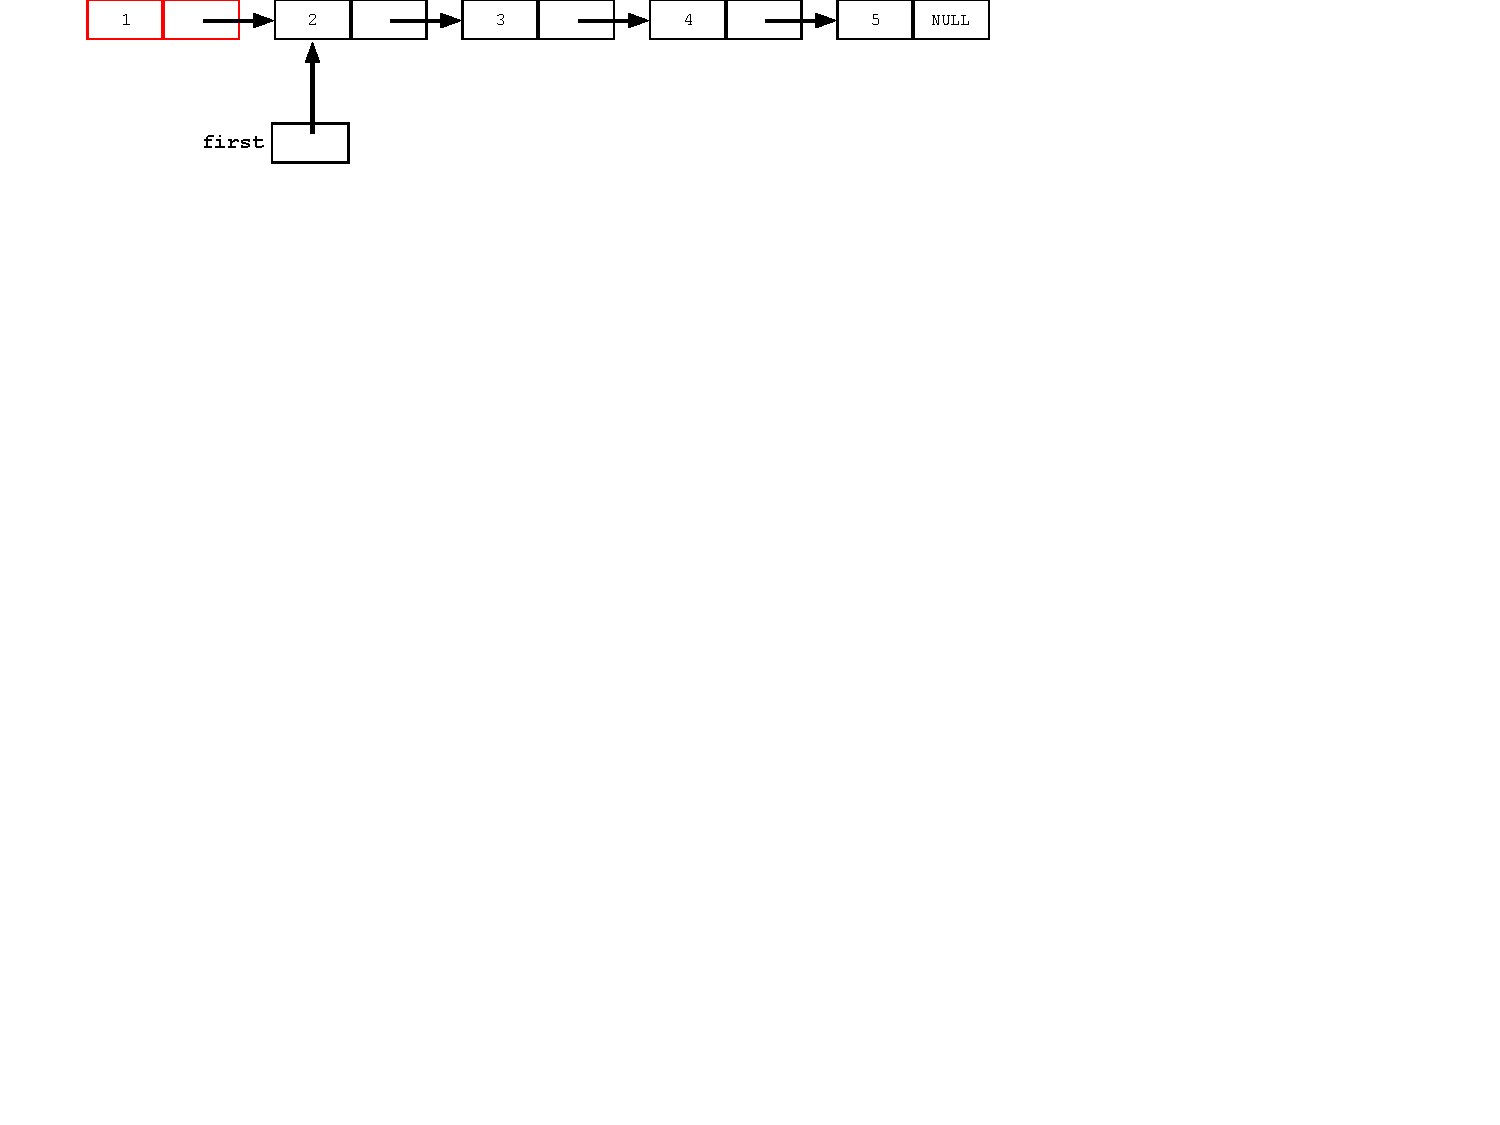
\includegraphics[width=14.0cm]{images/06_ll_pop}

\end{frame}


\begin{frame}[fragile]
\frametitle{Pop}

\begin{flushleft}
\relscale{0.75}
\begin{lstlisting}
box *save = first;
first=first->next;
delete save;
\end{lstlisting}  
\end{flushleft}


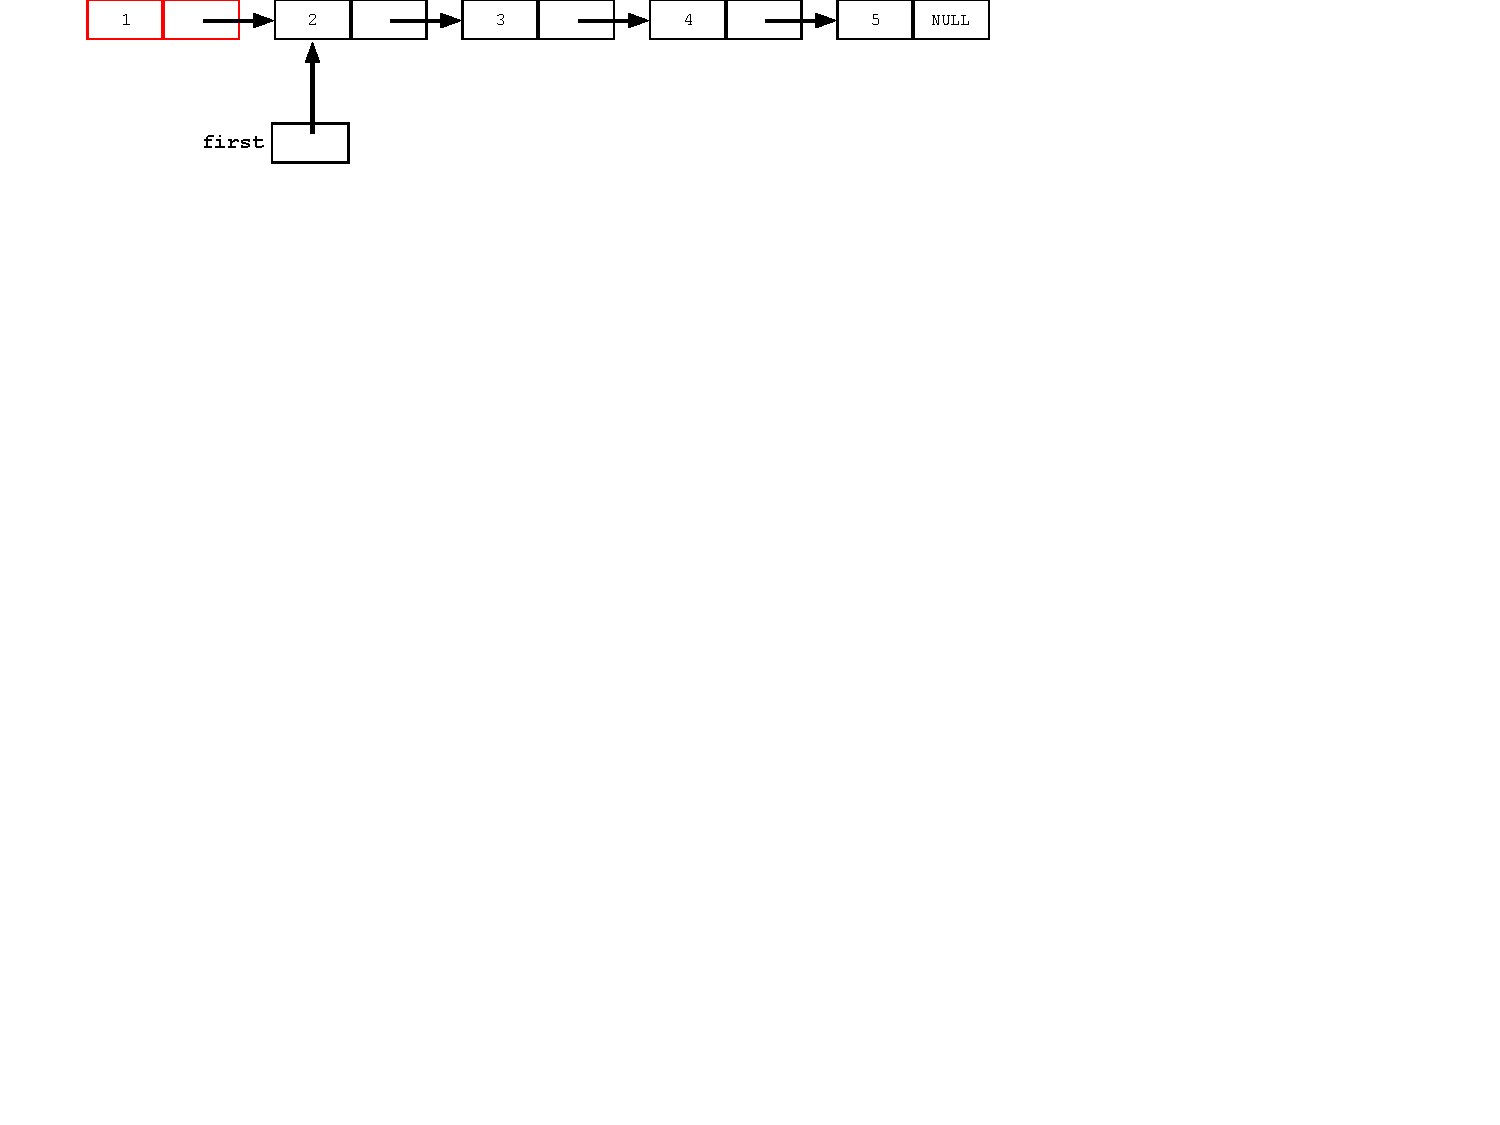
\includegraphics[width=14.0cm]{images/06_ll_pop}

\end{frame}


\begin{frame}
\centerline{Изтриване на елемент от позиция}
\end{frame}




\begin{frame}[fragile]
\frametitle{Изтриване}

\begin{flushleft}
\relscale{0.75}
\begin{lstlisting}
crr=...
\end{lstlisting}  
\end{flushleft}


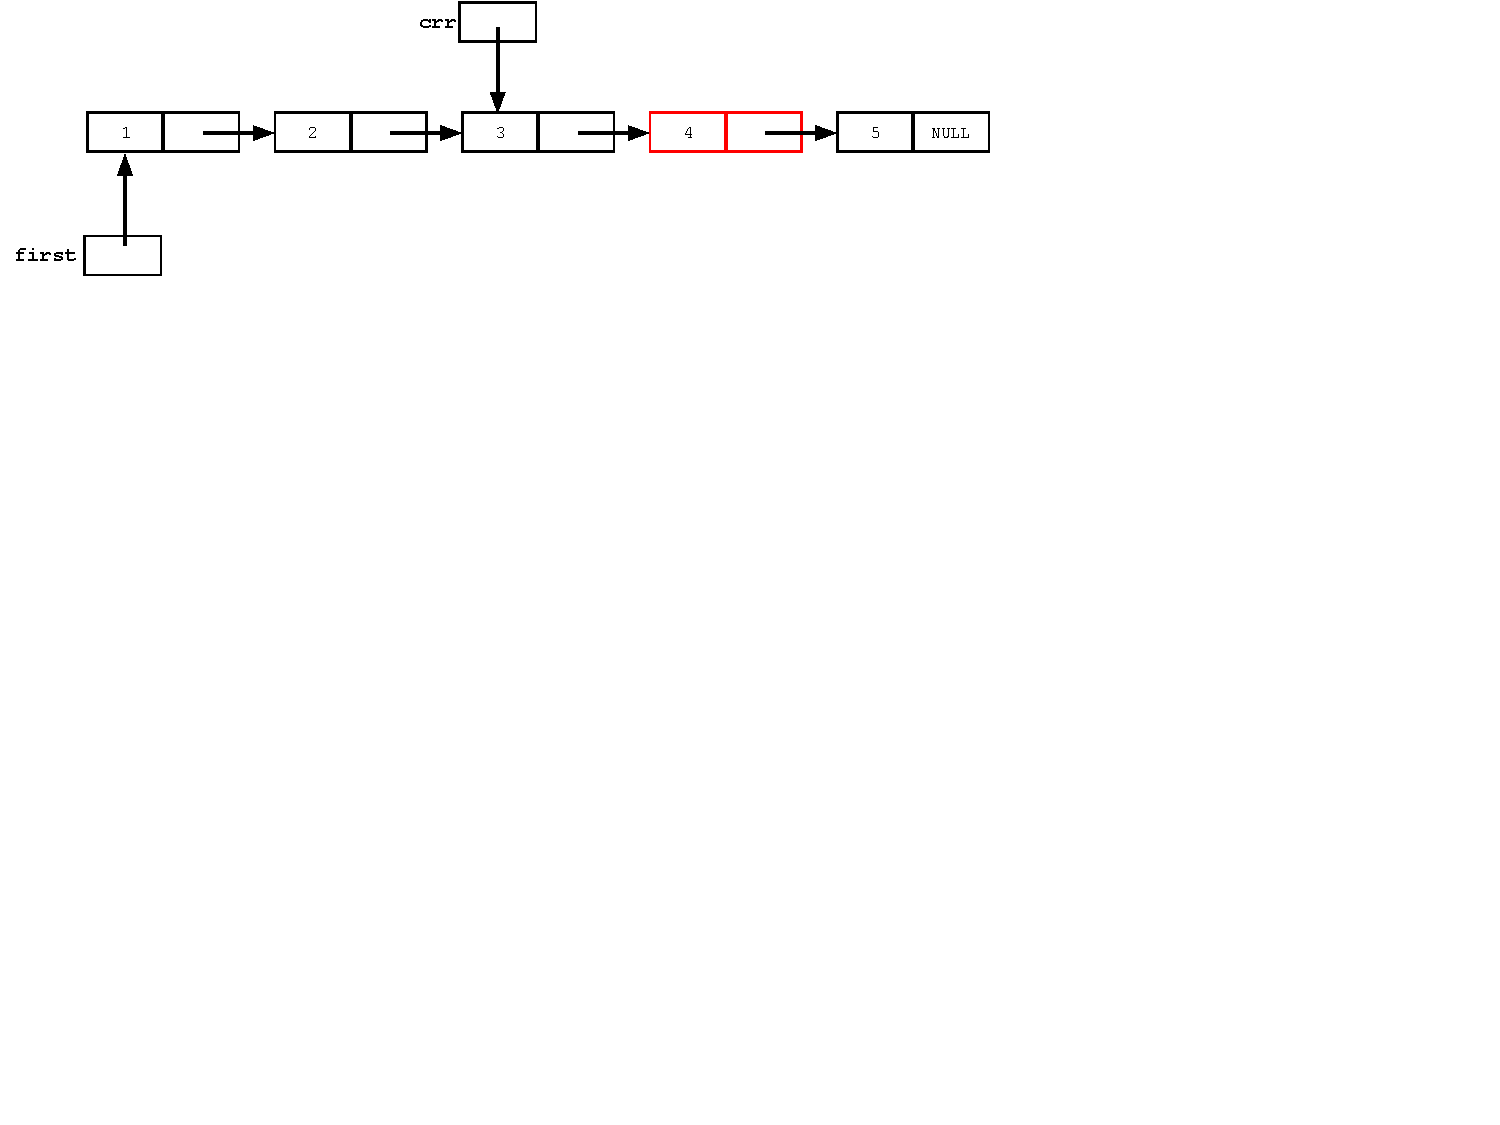
\includegraphics[width=14.0cm]{images/07_ll_remove_stepone}

\end{frame}


\begin{frame}[fragile]
\frametitle{Изтриване}

\begin{flushleft}
\relscale{0.75}
\begin{lstlisting}
box *save = crr->next;
\end{lstlisting}  
\end{flushleft}


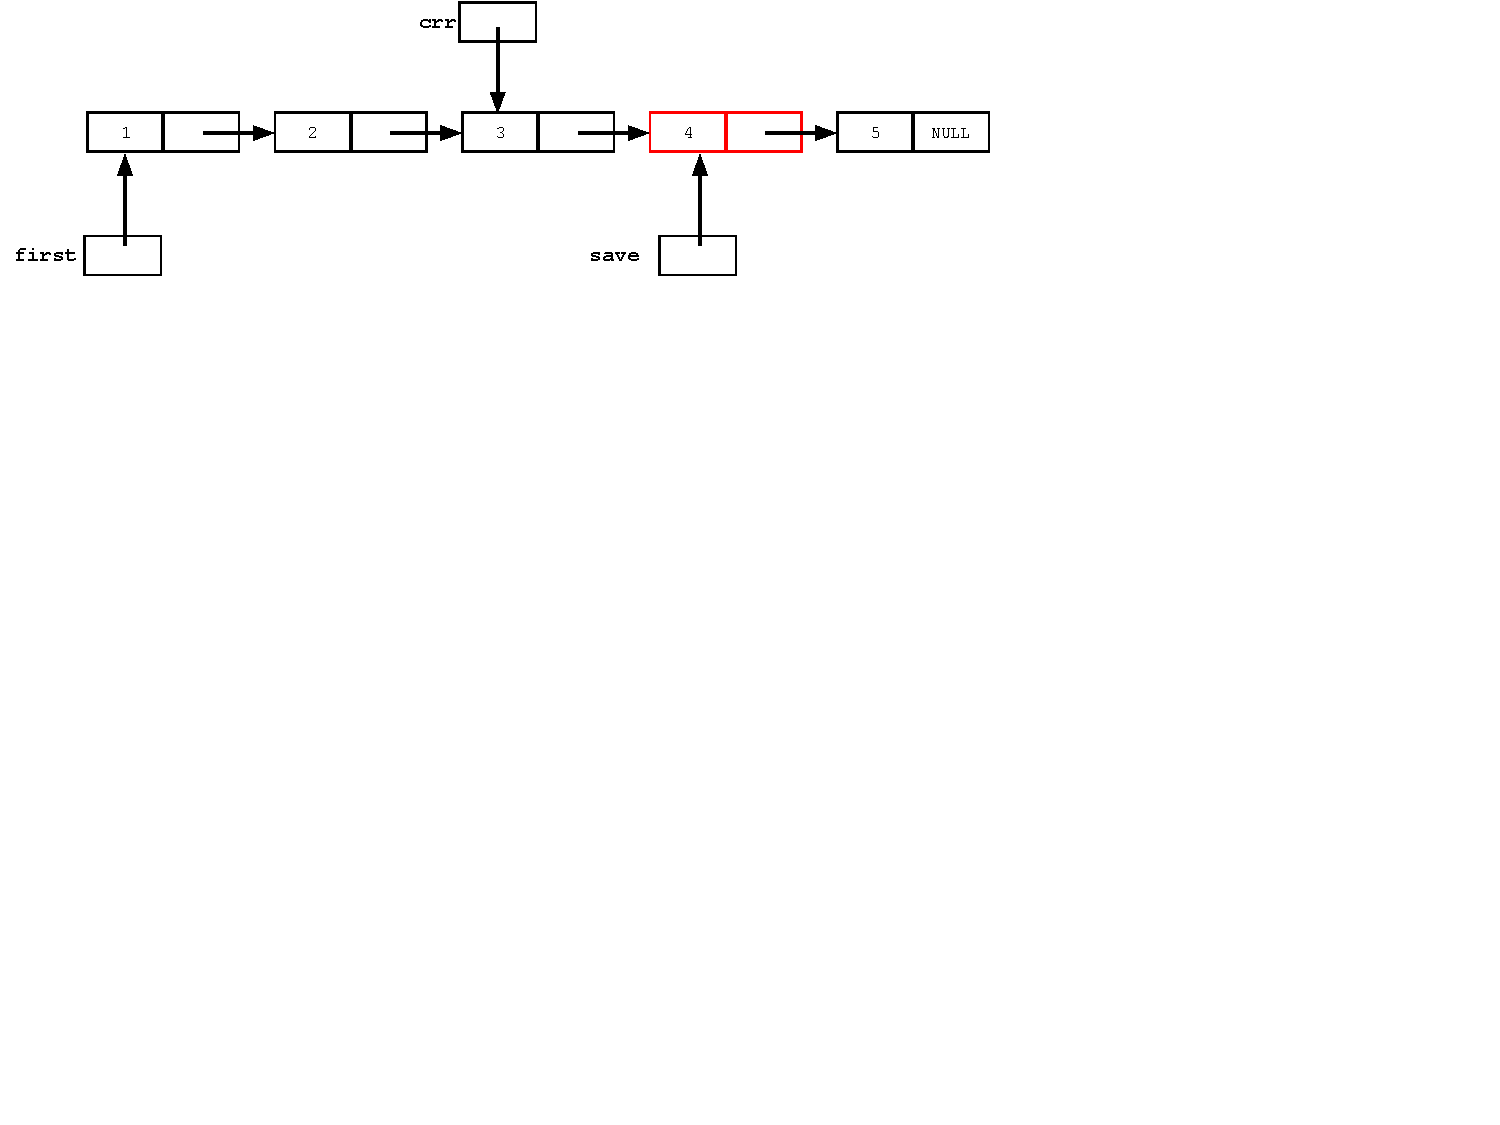
\includegraphics[width=14.0cm]{images/07_ll_remove_save}

\end{frame}


\begin{frame}[fragile]
\frametitle{Изтриване}

\begin{flushleft}
\relscale{0.75}
\begin{lstlisting}
box *save = crr->next;
crr->next = crr->next->next;
\end{lstlisting}  
\end{flushleft}


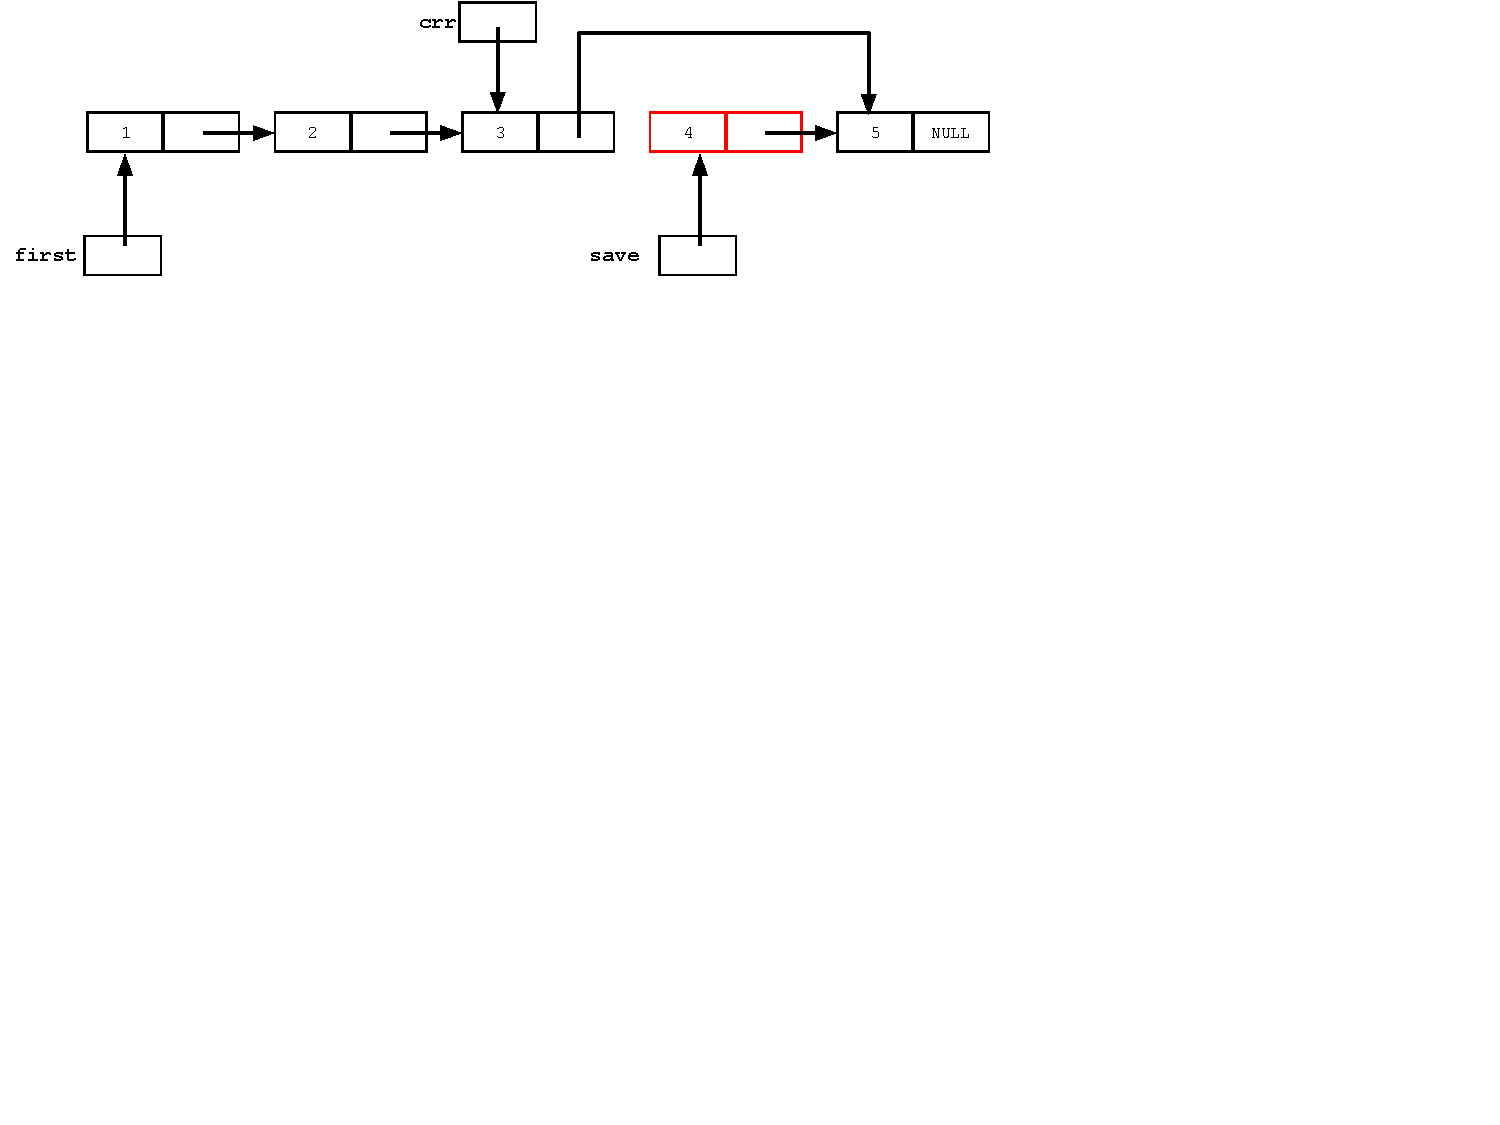
\includegraphics[width=14.0cm]{images/07_ll_remove_skip}

\end{frame}


\begin{frame}[fragile]
\frametitle{Изтриване}

\begin{flushleft}
\relscale{0.75}
\begin{lstlisting}
box *save = crr->next;
crr->next = crr->next->next;
delete save;
\end{lstlisting}  
\end{flushleft}


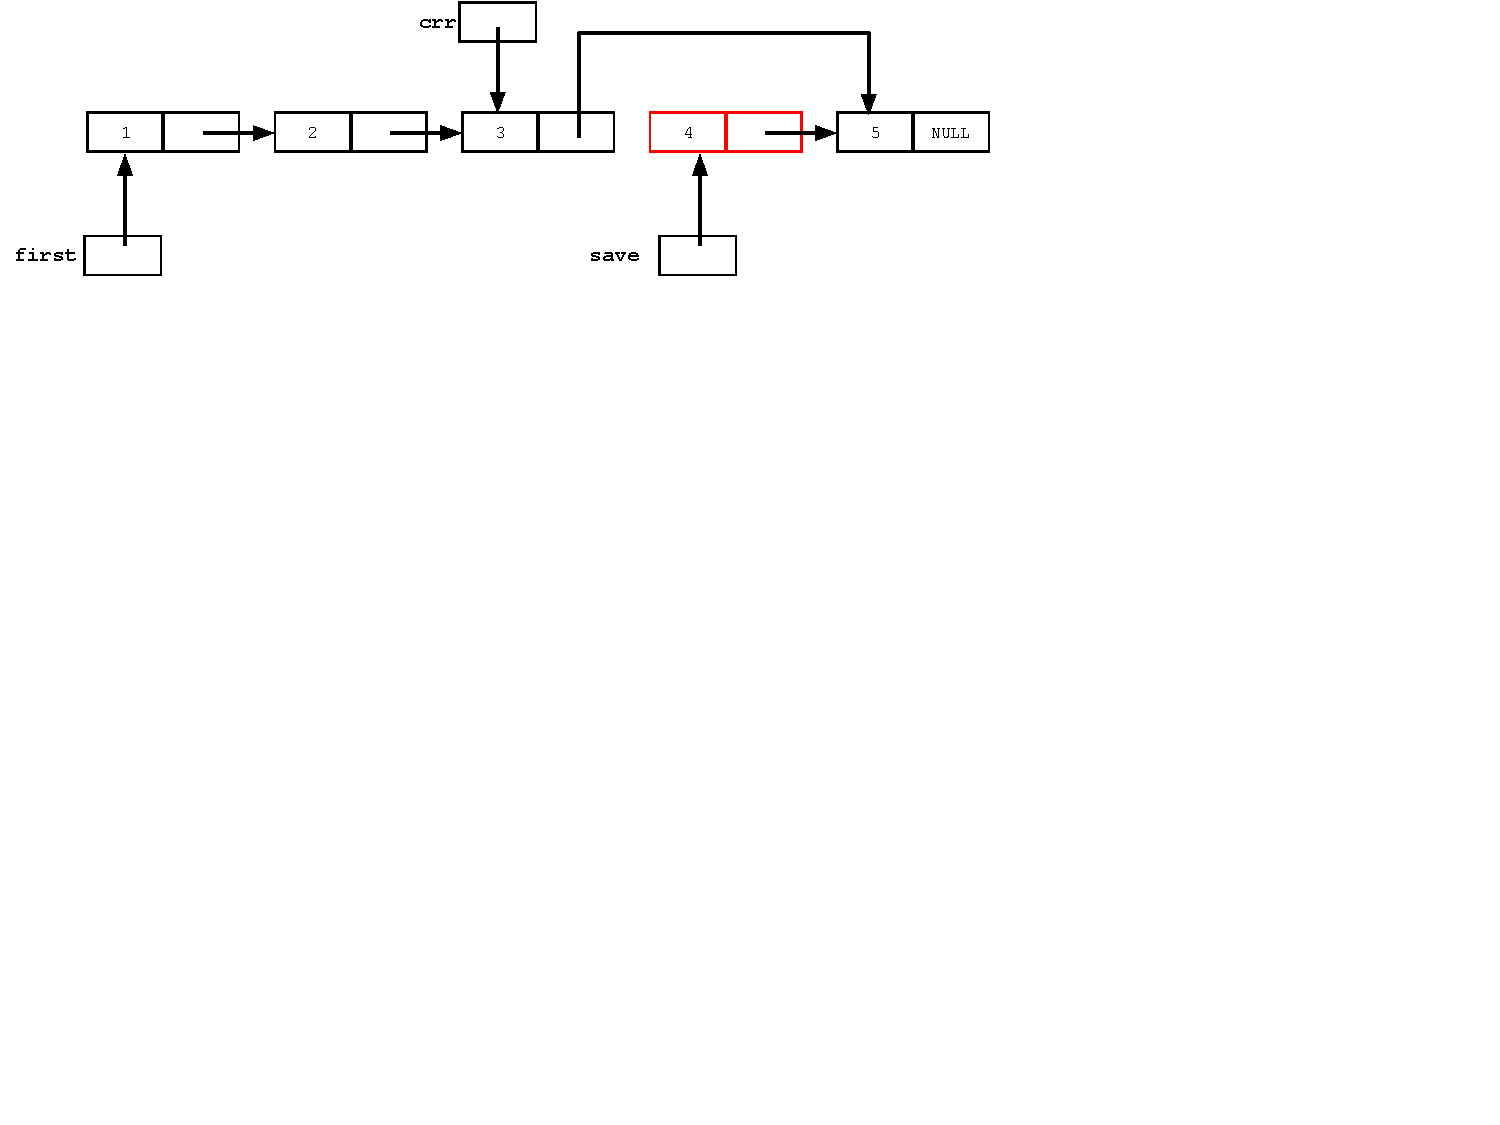
\includegraphics[width=14.0cm]{images/07_ll_remove_skip}

\end{frame}




\begin{frame}[fragile]
\frametitle{Изтриване на ел. 4}

\begin{flushleft}
\relscale{0.75}
\begin{lstlisting}
box *crr = first;
while (crr->next->data != 4)
  crr = crr->next;

box *save = crr->next;
crr->next = crr->next->next;
delete save;
\end{lstlisting}  
\end{flushleft}


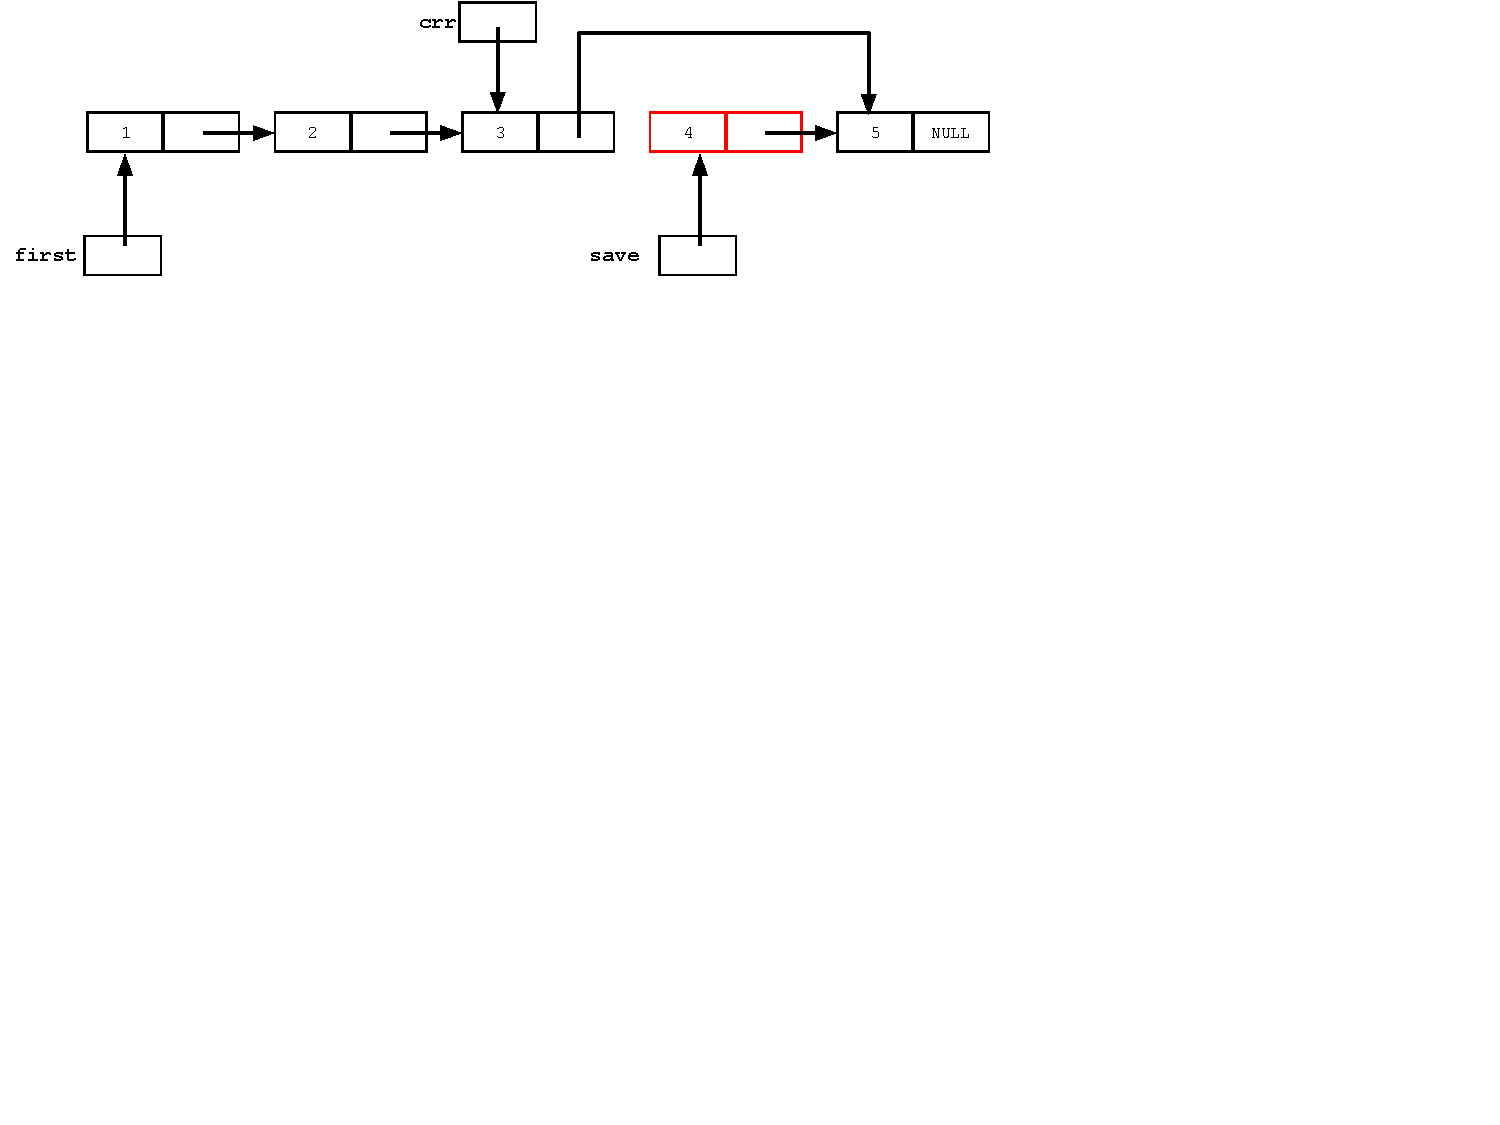
\includegraphics[width=14.0cm]{images/07_ll_remove_skip}

\end{frame}


\begin{frame}
\centerline{Благодаря ви за вниманието!}
\end{frame}

\end{document}



\begin{columns}[t]
  \begin{column}{0.55\textwidth}

  \end{column}
  \begin{column}{0.45\textwidth}

  \end{column}
\end{columns}
